% A Q&A chapter available in this template can help you when you want to change settings or need examples of how to get what you want.

\documentclass[	11pt,				% Font size
				twoside,			% Comment if you want to print on one side
				openright,
				headsepline,		% Adds a line under the page header
				headings=small,		% Defines sizing of the headers
				numbers=noenddot,	% No point at the right side of the section number
				%draft=false,
				BCOR=15mm,			% Absolute value of the binding correction.
				DIV=10, 			% larger value --> larger use of the page
				%captions=tableheading,
				paper=a4,			% only change if you want  another paper size
				abstracton,
				]{scrreprt}
				

%-----------------------------------------------------------------------------
% Document toggles for automatic adaptation of the document type
%-----------------------------------------------------------------------------
\usepackage{etoolbox}	% Makes it possible to really code in LaTeX
% Defining toggles
\newtoggle{dissertation}
\newtoggle{thesis}
\newtoggle{ingerman}
\newtoggle{nobinding}
\newtoggle{boldcaptions}

%%%%%%%%%%%%%%%%%%%%%%%%%%%%%%%%%%%%%%%%%%%%%%%%%%%%%%%%%%%%%%%%%%%%%%%%%%%%%%%%%%%%%%%%%%%% 
%TODO Setting values for toggles - Change here to modify the document layout to your needs %
%%%%%%%%%%%%%%%%%%%%%%%%%%%%%%%%%%%%%%%%%%%%%%%%%%%%%%%%%%%%%%%%%%%%%%%%%%%%%%%%%%%%%%%%%%%%

%%% Main properties %%%
\togglefalse{dissertation}		%if true (\toggletrue{dissertation}): no cover page
\toggletrue{thesis}				%if true (\toggletrue{thesis}): master or bachelor thesis (set false if \toggletrue{dissertation})
\toggletrue{ingerman}			%if \toggletrue{ingerman}: german if \togglefalse{ingerman}: english

%%% Secondary properties %%% 
\togglefalse{nobinding}		%if true: page layout is centered	
\toggletrue{boldcaptions}  	%if true: Fig. and Tab. are bold

%For oneside print: comment twoside in documentclass (line 4)






%%%%%%%%%%%%%%%%%%%%%%%%%%%%%%%%%%%%%%%%%
%%%% Settings - depending on toggles %%%%

%-----------------------------------------------------------------------------
% Language selection and translation definitions
%-----------------------------------------------------------------------------
% Depending on if german is selected as the main language, this part defines the main and secondary languages in the document and defines correct titles accordingly.
\iftoggle{ingerman}{%
	\newcommand{\mainLanguage}{ngerman}
	\newcommand{\secondLanguage}{english}
	\newcommand{\abstractMain}{Kurzfassung}
	\newcommand{\abstractSecond}{Abstract}
	\newcommand{\listOfFigures}{Abbildungsverzeichnis}
	\newcommand{\listOfTables}{Tabellenverzeichnis}
	\newcommand{\nomenclatureName}{Nomenklatur}
	\newcommand{\appendixName}{Anhang}
	\newcommand{\GreekSymbols}{Griechische Formelzeichen}
	\newcommand{\RomanSymbols}{Formelzeichen und Einheiten}
	\newcommand{\abbreviations}{Abk\"urzungen}
	\newcommand{\subscripts}{Indizes}
	\newcommand{\Literaturename}{Literaturverzeichnis}
}%{%
%	\newcommand{\mainLanguage}{english}
%	\newcommand{\secondLanguage}{ngerman}
%	\newcommand{\abstractMain}{Abstract}
%	\newcommand{\abstractSecond}{Kurzfassung}
%	\newcommand{\listOfFigures}{List of Figures}
%	\newcommand{\listOfTables}{List of Tables}
%	\newcommand{\nomenclatureName}{Nomenclature}
%	\newcommand{\appendixName}{Appendix}
%	\newcommand{\GreekSymbols}{Greek Symbols}
%	\newcommand{\RomanSymbols}{Roman Symbols}
%	\newcommand{\abbreviations}{Abbreviations}
%	\newcommand{\subscripts}{Subscripts}
%	\newcommand{\Literaturename}{Literature}
%}


%-----------------------------------------------------------------------------
% Page layout (margins, headers and footers)
%-----------------------------------------------------------------------------
\usepackage{geometry}
%\usepackage{scrlayer-scrpage} % Package to control headers and footers more comprehensive
%\pagestyle{scrheadings} % To automatically format headers and footers well when having two page print and different left and right margins

\newtoggle{onesideprint}
\makeatletter
	\if@twoside
		\togglefalse{onesideprint}
	\else
		\toggletrue{onesideprint}
	\fi
\makeatother

\interfootnotelinepenalty=10000 % Prevents the footnotes to split in two pages

\newlength{\lmargin}
\newlength{\rmargin}
\newlength{\tmargin}
\newlength{\bmargin}

% Defining page margins for different document types
	%page width
\iftoggle{nobinding}{
	\iftoggle{dissertation}{
		\setlength{\lmargin}{27mm}
		\setlength{\rmargin}{27mm}
	}{}
	\iftoggle{thesis}{
		\setlength{\lmargin}{27.5mm}
		\setlength{\rmargin}{27.5mm}
	}{}
}{	\iftoggle{onesideprint}{                % If with binding and one page print
		\iftoggle{dissertation}{
			\setlength{\lmargin}{30mm}
			\setlength{\rmargin}{24mm}
		}{}
		\iftoggle{thesis}{
			\setlength{\lmargin}{30mm}
			\setlength{\rmargin}{25mm}
		}{}
		}{                                  % If with binding and two page print
		\iftoggle{dissertation}{
			\setlength{\lmargin}{24mm}
			\setlength{\rmargin}{30mm}
		}{}
		\iftoggle{thesis}{
			\setlength{\lmargin}{25mm}
			\setlength{\rmargin}{30mm}
	}{}}
}
	%page height
\iftoggle{dissertation}{
	\setlength{\tmargin}{35mm}
	\setlength{\bmargin}{35mm}
}{}
\iftoggle{thesis}{
	\setlength{\tmargin}{37mm}
	\setlength{\bmargin}{38mm}
}{}

% Setting the page margins
\geometry{a4paper, left=\lmargin, right=\rmargin, top=\tmargin, bottom=\bmargin}

\newlength{\offsetCoverPage}
\newlength{\marginCoverPage}
\iftoggle{onesideprint}{%
	\setlength{\offsetCoverPage}{-1mm}
	\setlength{\marginCoverPage}{0mm}

}{%
	\setlength{\offsetCoverPage}{0mm}
	\setlength{\marginCoverPage}{0.25mm}
}

%% Setting header and footers
\usepackage{fancyhdr}	% This package is easier to control than the already implemented header and footer controls in the Koma-Script class
\pagestyle{fancy}

\renewcommand{\sectionmark}[1]{\normalsize\markright{\thesection\ #1}{}}
\renewcommand{\chaptermark}[1]{\normalsize\markboth{\thechapter\ #1}{}}
\lhead{\leftmark}
\chead{}
\rhead{\rightmark}

%-----------------------------------------------------------------------------
% Base packages
%-----------------------------------------------------------------------------
\usepackage[T1]{fontenc}	 % Enables font encoding for accented characters
\usepackage[utf8]{inputenc}  % Enables input of accented characters
\usepackage[english,ngerman]{babel}	% Defines the document language
\usepackage{ifpdf} 		
% This creates a true boolean if you are executing your code using PDFLatex or LuaLaTex, otherwise it is false. It helps later on to define correct package options for different compiling methods. (See PDF-Setup)

\usepackage{blindtext} % Just to create lorem ipsum text in this template
\usepackage{datetime}
\newdateformat{monthyeardate}{%
  \monthname[\THEMONTH] \THEYEAR}

% There exist several todo packages like todonotes, todo, or easy-todo.
% Choose one todo package and import it via the \usepackage{} command.



%-----------------------------------------------------------------------------
% Font properties
%-----------------------------------------------------------------------------
%\usepackage{fourier} %PDF-compatible font "Utopia". There exists a free look-alike: Heuristica
\usepackage{lmodern} % So that headings don't pixelate (bitmap font to vector font); Don't use it simultaneously with fourier (previous font, see more at issues 16 and 20)
\makeatletter % No warnings because of a replaced font
  \let\@font@info\@gobble
  \let\@font@warning\@gobble
\makeatother

\iftoggle{boldcaptions}{
	\renewcommand{\caplabelfont}{\bfseries} % Fig. and Tab. are bold
}{}


%-----------------------------------------------------------------------------
% Redefining bullet points
%-----------------------------------------------------------------------------
\AtBeginDocument{
  \renewcommand{\labelitemi}{\(\bullet\)}
  \renewcommand{\labelitemii}{\(\circ\)}
}


%-----------------------------------------------------------------------------
% Line and paragraph spacing
%-----------------------------------------------------------------------------
\usepackage{setspace} % Change Linespread
\onehalfspacing % Linespread 1.5
\setlength\parskip{\medskipamount} % Small linespread between two paragraphs
\setlength\parindent{0pt} % No indentation in the first line of a new paragraph


%-----------------------------------------------------------------------------
% Color definitions
%-----------------------------------------------------------------------------
\usepackage{xcolor}
% The standart ERC colors (dark variant)
% Check sharepoint for lighter variants if needed
\definecolor{ercred}{RGB}{229,48,39}	% Color of the ERC logo
\definecolor{ercblue}{RGB}{16, 88, 176}
\definecolor{ercorange}{RGB}{244, 115, 40}
\definecolor{ercviolett}{RGB}{95, 55, 155}
\definecolor{ercdarkred}{RGB}{155, 35, 30}
\definecolor{ercpink}{RGB}{190, 65, 152}
\definecolor{ercdarkgreen}{RGB}{0, 135, 70}

% The official RWTH colors
% Check official document for lighter colors if needed
\definecolor{rwthblue}{RGB}{0,84,159}
\definecolor{rwthblack}{RGB}{0,0,0}
\definecolor{rwthmagenta}{RGB}{227,0,102}
\definecolor{rwthyellow}{RGB}{255,237,0}
\definecolor{rwthpetrol}{RGB}{0,97,101}
\definecolor{rwthturquoise}{RGB}{0,152,161}
\definecolor{rwthgreen}{RGB}{87,171,39}
\definecolor{rwthmaygreen}{RGB}{189,205,0}
\definecolor{rwthorange}{RGB}{246,168,0}
\definecolor{rwthred}{RGB}{204,7,30}
\definecolor{rwthbordeaux}{RGB}{161,16,53}
\definecolor{rwthviolett}{RGB}{97,33,88}
\definecolor{rwthlila}{RGB}{122,11,172}

% Color aliases
% Use these in the document to be able to switch easily
\colorlet{color0}{ercred}
\colorlet{color1}{ercblue}
\colorlet{color2}{ercorange}
\colorlet{color3}{ercviolett}
\colorlet{color4}{ercdarkred}
\colorlet{color5}{ercpink}
\colorlet{color6}{ercdarkgreen}

%-----------------------------------------------------------------------------
% List environments
%-----------------------------------------------------------------------------
\usepackage{enumitem}
% This provides more user control over the list environments. Here you can create your own enumeration format, etc. (See Q&A Environment Setup as an example)


%-----------------------------------------------------------------------------
% Style formats 
%-----------------------------------------------------------------------------
\usepackage{listings}
% This enables writing programming code as written in a programming environment in LaTeX.

\lstset{literate=%
    {ä}{{\"a}}1
    {Ä}{{\"A}}1
    {ö}{{\"o}}1
    {Ö}{{\"O}}1
    {ü}{{\"u}}1
    {Ü}{{\"Ü}}1
    {ß}{{\ss}}1
}
% Adds the possibility to include german special charachters in the lstlisting.

\usepackage{textcomp} % Is needed, if "\usepackage{lmodern}" is used (Line 195)
\usepackage{Resources/ModelicaStyle}	% Modelica style file

%-----------------------------------------------------------------------------
% Nomenclature
%-----------------------------------------------------------------------------
\usepackage[intoc]{nomencl}		% Used for automatic generation of nomenclature
\RequirePackage{ifthen}			% Checks if ifthen functions
% Defines the nomenclature sections
\renewcommand{\nomgroup}[1]{%
	\ifthenelse{\equal{#1}{G}}{\item[\newline\textbf{\GreekSymbols}]}{
	\ifthenelse{\equal{#1}{U}}{\item[\newline\textbf{\subscripts}]}{
	\ifthenelse{\equal{#1}{A}}{\item[\newline\textbf{\abbreviations}]}{
	\ifthenelse{\equal{#1}{S}}{\item[\newline\textbf{\RomanSymbols}]}{
	\ifthenelse{\equal{#1}{Y}}{\item[\newline\textbf{Codes used for configurations of simulation}]}{
}}}}}
}
% Changing some of the spacings
\newcommand{\nomunit}[1]{%
\renewcommand{\nomentryend}{\hspace*{\fill}#1}%
}
\renewcommand{\nomlabel}[1]{\hspace{2.5em}#1}
\makenomenclature
\setlength\nomlabelwidth{2.5cm}


%-----------------------------------------------------------------------------
% Mathematic
%-----------------------------------------------------------------------------
\usepackage{amsmath}
\usepackage{amssymb}
\usepackage{array}

\usepackage[version=4]{mhchem}


%-----------------------------------------------------------------------------
% Q&A environment setup
%-----------------------------------------------------------------------------
% The following commands are only used for the Q&A format in the examples of the template. You can remove this in your main document. Note that this is also useful for cerating exam formats, etc.
\newenvironment{QandA}{\begin{enumerate}[label=\bfseries\arabic*.]\bfseries}
                      {\end{enumerate}}
\newenvironment{answered}{\par\normalfont}{}


%-----------------------------------------------------------------------------
% PDF-Setup
%-----------------------------------------------------------------------------
\ifpdf
	%We use PDFLaTeX
	\usepackage[pdftex]{graphicx} 
	\pdfimageresolution=100
	\pdfminorversion=7
	\pdfcompresslevel=9
	\usepackage[pdftex,
		urlcolor=blue,
		linktoc=all,
		colorlinks=true,
		linkcolor=black,
		citecolor=black,
		pdfview=FitH,
		pdfstartview=FitH,
		plainpages=false]{hyperref}	% Allows cross references and hyperlinks
	\hypersetup{
		pdfauthor={Your Name here},
        pdftitle={Name of your thesis},
        pdfsubject={},
        pdfkeywords={several helpful keywords},
        pdfproducer={LaTeX with hyperref},
        pdfcreator={pdflatex}}
    \usepackage[figure,figure*]{hypcap}
\else
	%DVI oder PS Ausgabe
	\usepackage{graphicx} 
\fi
%\usepackage{pdfpages}	
% Simplifies the inclusion of whole PDF-Pages, e.g. cover page. Should be placed after "graphicx" package


%-----------------------------------------------------------------------------
% Units and symboles
%-----------------------------------------------------------------------------
\usepackage{siunitx}	
% Prefered to package "siunits". Should be placed after "graphicx" package

\usepackage[official]{eurosym}
\DeclareUnicodeCharacter{20AC}{\euro} 
% The normale euro symbol via [Alt Gr][€] is replaced by a high quality one

%-----------------------------------------------------------------------------
% General floats
%-----------------------------------------------------------------------------
\usepackage{float}
\usepackage{placeins}	% Allows more control of the floats, e.g. \FloatBarrier
\usepackage{caption}	
\usepackage{subcaption}	% Allows manipulation of caption entries in lists

%-----------------------------------------------------------------------------
% Figures
%-----------------------------------------------------------------------------
\graphicspath{{Figures/}}	% Defining where the figure are located (for pdf_tex).

\usepackage{tikz,pgfplots} \pgfplotsset{compat=newest}
% Allows using TikZ plots with the newest package available
\usetikzlibrary{plotmarks, shapes, arrows, positioning, shadows, trees}
% plotmarks is used in the diagrams, other values are for flow charts, etc.

%\usetikzlibrary{external}	% Uncomment to activate external TikZ compliation
%\tikzexternalize[prefix=Figures/TikZ]	% Uncomment to place external tikZ files in a separate folder.

\newlength\figureheight 
\newlength\figurewidth 
% Defining the length and height variables of the TikZ plots


%-----------------------------------------------------------------------------
% Tables
%-----------------------------------------------------------------------------
\usepackage{longtable}	% For tables longer than a page
\usepackage{multirow}	% Allows multirow in tables
\usepackage{multicol}	% Allows multicolumn in tables
\usepackage{booktabs}	% Better horizontal lines in tables \toprule \midrule ...

\usepackage{dcolumn} 	% Allows allignment by decimal point
  \newcolumntype{d}[1]{D{.}{.}{#1}}	% Defining some new formats
  \newcolumntype{C}[1]{>{\centering\let\newline\\\arraybackslash\hspace{0pt}}m{#1}}



%-----------------------------------------------------------------------------
% References and Citations
%-----------------------------------------------------------------------------
\usepackage{varioref}
\usepackage[square]{natbib}
\usepackage{bibunits}


%-----------------------------------------------------------------------------
% Manually added packages
%-----------------------------------------------------------------------------
%\usepackage{anything}


%%%%%%%%%%%%%%%%%%%%%%%%%%%%%%%%%%%%%%%%%%%%%%%%%%%%%%%%%%%%%%%%%%%%%%%%%%%%%%
%-----------------------------------------------------------------------------
% DOCUMENT BEGINS HERE!
%-----------------------------------------------------------------------------
%%%%%%%%%%%%%%%%%%%%%%%%%%%%%%%%%%%%%%%%%%%%%%%%%%%%%%%%%%%%%%%%%%%%%%%%%%%%%%

\begin{document}


\pagestyle{empty}
\newcounter{Hilfszaehler}

\expandafter\selectlanguage\expandafter{\mainLanguage}

\cleardoublepage
\pagenumbering{Roman} % roman page numbers


%-----------------------------------------------------------------------------
% Cover page
%-----------------------------------------------------------------------------
% Based on the document type and language, the template decides if and which cover page should be used and includes it in the final document.

\iftoggle{thesis}{%
	\iftoggle{ingerman}{%
		\begin{titlepage}
\begin{addmargin}{\offsetCoverPage} 
%TODO Um das RWTH-Logo zu benutzen, musst du das Formblatt RWTH-Logo Deutsch aus der Datei Formulare.txt
%TODO ausfüllen und es dem ZPA schicken!

%-----------------------------------------------------------------------------
% Platzierung der Kopfzeile(Nummer und Logo)
%-----------------------------------------------------------------------------
\setlength{\unitlength}{1cm}
\begin{picture}(0,0)
\put(7.977,0.68){
\includegraphics[width = 0.5\textwidth]{Resources/rwth_eerc_rgb_ohne_Schutzraum.pdf}}
%TODO Ändere die Nummer deiner Arbeit, und wenn noetig die Bezeichnung(BA, MA, PA)
%TODO Die Abkürzungen sind Deutsch, auch wenn die Arbeit in Englisch verfasst wird
\put(0,1.32){\fontfamily{phv}\selectfont\huge{BA 280}}
\end{picture}
\end{addmargin}
%-----------------------------------------------------------------------------
% Titel deiner Arbeit
%-----------------------------------------------------------------------------
\addvspace{2.6cm}
%TODO Formaenderung des Titels
\begin{addmargin}[\marginCoverPage]{0cm}
\begin{center}
{\fontfamily{phv}\selectfont\huge Bachelorarbeit} 
\end{center}

{\Large \par}
\addvspace{1.5cm}
\begin{center}
%TODO Wenn du ein "Sperrvermerk" für deine Arbeit brauchst, entferne den Kommentar in der naechsten Zeile
%\textbf{{\color{ercred}\fontfamily{phv}\selectfont{\huge Sperrvermerk}}}\\

%TODO  Der Englische Titel deiner Arbeit wird nach dem "\huge" in der naechsten Zeile geaendert
\textbf{\fontfamily{phv}\selectfont{\huge Modellierung und Simulation des Wasserstoff-Energiesystems eines Quarzglasherstellers in Modelica zur Identifikation effizienter Systemkonzepte}}
\end{center}

\addvspace{1.5cm}
\begin{center}
%TODO Falls der deutsche Name noch noetig ist, kommt er in die naechste Zeile
{\fontfamily{phv}\selectfont Modelling and simulation of the hydrogen-energysystem of a fused quartz producer in Modelica to identify efficient systemconcepts}
\end{center}

%-----------------------------------------------------------------------------
% Namen, Daten
%-----------------------------------------------------------------------------
\vfill
\begin{center}
\begingroup
\fontfamily{phv}\selectfont
%TODO Bitte aendere das Datum deiner Abgabe
Aachen, \monthyeardate\today \\
\addvspace{0.5cm}
%TODO Bitte aendere deinen Namen und Matrikelnummer in den naechsten beiden Zeilen
\textbf{Tobias Jonathan Boschmann} \\
Matrikelnummer: 379947 \\
\addvspace{0.5cm}
%TODO Deine Betreuer. Achte auf die richtige Schreibweise des Titels.
Betreuer:\\
Hannah Krützfeldt, M. Sc. \\
Univ.-Prof. Dr.-Ing. Dirk Müller \\
\addvspace{0.5cm}
%TODO  Eingabe der richtigen Anschrift des Instituts.
Diese Arbeit wurde vorgelegt am:\\
E.ON Energy Research Center | ERC \\
Institute for Energy Efficient Buildings and Indoor Climate | EBC\\
(Lehrstuhl für Gebäude- und Raumklimatechnik)\\
Mathieustraße 10, 52074 Aachen\\
\endgroup
\end{center}
\end{addmargin}
\end{titlepage}


	}{%
		\begin{titlepage}
\begin{addmargin}{\offsetCoverPage}
%TODO To use the RWTH Aachen Logo you are required to complete the form
%TODO RWTH-Logo Englisch in the file Formulare.txt and submit it to the Central Examination Offices

%-----------------------------------------------------------------------------
% Place the header (Logo and number of thesis)
%-----------------------------------------------------------------------------
\setlength{\unitlength}{1cm}
\begin{picture}(0,0)
\put(7.977,0.68){
\includegraphics[width = 0.5\textwidth]{Resources/rwth_eerc_rgb_ohne_Schutzraum}}
%TODO Change the number of your thesis, and if necessary the abbreviation (BA, MA, PA)
%TODO The abbreviation are German, also if you thesis is written in English
\put(0,1.32){\fontfamily{phv}\selectfont\huge{MA 000}}
\end{picture}
\end{addmargin}
%-----------------------------------------------------------------------------
% Title of your Thesis
%-----------------------------------------------------------------------------
\addvspace{2.6cm}
%TODO Change the kind of your thesis accordingly
\begin{addmargin}[\marginCoverPage]{0cm}
\begin{center}
{\fontfamily{phv}\selectfont\huge Master's Thesis} 
\end{center}

{\Large \par}
\addvspace{1.5cm}
\begin{center}
%TODO If you need a "Sperrvermerk" on your thesis, uncomment the next line 
%\textbf{{\color{ercred}\fontfamily{phv}\selectfont{\huge Sperrvermerk}}}\\

%TODO  Title of your thesis goes into the next line, after the \huge
\textbf{\fontfamily{phv}\selectfont{\huge Design of Master's thesis }}
\end{center}

\addvspace{1.5cm}
\begin{center}
%TODO And here goes the German title of your thesis. Should be in your papers.
{\fontfamily{phv}\selectfont Design von Bachelorarbeiten}
\end{center}

%-----------------------------------------------------------------------------
% Dates, Names... .
%-----------------------------------------------------------------------------
\vfill
\begin{center}
\begingroup
\fontfamily{phv}\selectfont
%TODO Please update the date of submission
Aachen, \monthyeardate\today \\
\addvspace{0.5cm}
%TODO  Your Name Here (and in the next line your matriculation number
\textbf{Your Name} \\
Matriculation number: 000815 \\
\addvspace{0.5cm}
%TODO Your supervisor. Make sure you get her academic title right, most of them aren't physicist. 
Supervisors:\\
Max Mustermännin, M.Sc. \\
Univ.-Prof. Dr.-Ing. Dirk Müller \\
\addvspace{0.5cm}
%TODO  Enter correct date here
The present work was submitted to the:\\
E.ON Energy Research Center | ERC \\
Institute for Energy Efficient Buildings and Indoor Climate | EBC\\
Mathieustrasse 10, 52074 Aachen, Germany\\
\endgroup
\end{center}
\end{addmargin}
\end{titlepage}


	}
}{}
\iftoggle{dissertation}{%
	\begin{titlepage}

\vspace*{-3cm}

\begin{picture}(0,0)
%\put(350,-50){\includegraphics[height=2.5cm]{Figures/cover/EERC_EBC_Logo_RGB.jpg}}
%\put(350,-770){\includegraphics[height=1.27cm]{Pictures/RWTHAACHENUNIVERSITY_sw.png}} %Using the RWTH-Logo in a student thesis is not allowed!
%\put(0,5){\begin{minipage}[b]{3.0cm}
%\huge{} % Hier Nummer der Bachelor- / Masterarbeit eintragen
%\end{minipage}}
\end{picture}

\vspace{3cm}
%\begin{center}{\textbf{\huge Dissertation}}\end{center}{\Large \par}

%\vspace{0.5cm}
%\begin{spacing}{2}
\begin{center}{"Dissertations are for true heroes"}\end{center}
%\end{spacing}
\begin{center}{"Dissertationen sind für wahre Helden"}\end{center}

%\begin{figure}[H]
%\begin{center}
%\includegraphics[height=6cm]{Pictures/PCM_Slurry1.jpg} % Hier Bild einfügen, Höhe 6cm!
%\end{center}
%\end{figure}

\vspace{1cm} % Falls kein Bild: diesen Platzhalter statt der Figure-Umgebung

\begin{center}{Der Fakultät für Maschinenwesen der Rheinisch-Westfälischen Technischen Hochschule
Aachen vorgelegte Dissertation zur Erlangung des akademischen Grades eines Doktors der Ingenieurwissenschaften\\
\vspace{1cm}
von \\
\vspace{0.5cm}
Dein Name}\end{center}%{\large \par}

\Large

\begin{center}
%\textbf{Kristian Huchtemann} \\\medskip 
%\large
%matriculation number: 3XXXXX \\\medskip
%\vspace{0.5cm}
%Supervisors:\\
%Super Supervisor, M.Sc. \\
%Univ.-Prof. Dr.-Ing. Dirk Müller \\\vspace{1.0cm}


%RWTH~Aachen~University\\
%E.ON Energy Research Center | ERC \\
%Institute for Energy Efficient Buildings and Indoor Climate | EBC \\
%Mathieustraße 10, D-52074 Aachen\\
\end{center}

\end{titlepage}

	\thispagestyle{empty}
\cleardoublepage\textbf{}

\begin{titlepage}

\vspace*{-3cm}

\vspace{3cm}
%\begin{center}{\textbf{\huge Dissertation}}\end{center}{\Large \par}

%\vspace{0.5cm}
%\begin{spacing}{2}
\begin{center}\large{Dissertations are for true heroes}\end{center}
%\end{spacing}

\vspace{0.8 cm}

\begin{center}{``Dissertationen sind für wahre Helden''}\end{center}

%\begin{figure}[H]
%\begin{center}
%\includegraphics[height=6cm]{Pictures/PCM_Slurry1.jpg} % Hier Bild einfügen, Höhe 6cm!
%\end{center}
%\end{figure}

\vspace{0.8cm} % Falls kein Bild: diesen Platzhalter statt der Figure-Umgebung

\begin{center}\small{\textsf{Von der Fakultät für Maschinenwesen der Rheinisch-Westfälischen Technischen Hochschule Aachen zur Erlangung des akademischen Grades eines Doktors der Ingenieurwissenschaften genehmigte Dissertation}}\\
\vspace{0.5cm}
\small{vorgelegt von} \\
\vspace{0.5cm}
\small{Dein Name}\end{center}%{\large \par}

\vspace{1.0cm}
\begin{tabbing}
\small{\textsf{Berichter:}} \= \small{\textsf{Univ.-Prof. Dr.-Ing. Dirk Müller}}\\
\>\small{\textsf{Professor Max Mustermann, Ph. D.}}\\ 
\end{tabbing}

%\vspace{0.2cm}
\small{\textsf{Tag der mündlichen Prüfung: 01. Januar 2030}}\\

\vspace{0.5cm}
\small{\textsf{Diese Dissertation ist auf den Internetseiten der Universitätsbibliothek online verfügbar.}}


\end{titlepage}
%\thispagestyle{empty}
%\cleardoublepage\textbf{}
%\thispagestyle{empty}

\begin{titlepage}
\vspace*{-3cm}

\vspace{3cm}
\begin{center}{Dein Name}\end{center}
\vspace{0.0cm}
\begin{center}{"Dissertations are for true heroes"}\end{center}
\end{titlepage}

}
\cleardoublepage

%-----------------------------------------------------------------------------
% Page numbers
%-----------------------------------------------------------------------------
\pagenumbering{Roman} % roman page numbers

\iftoggle{onesideprint}{
	\fancyfoot[C]{\thepage}
	\fancyfoot[LE,RO]{}}
	{
	\fancyfoot[LE,RO]{\thepage}
	\fancyfoot[C]{}
	}

%-----------------------------------------------------------------------------
% Abstract in English and German (Both are required)
%-----------------------------------------------------------------------------
% Different documents have different types of showing the title of the abstract, This part assigns the correct formmat to your document considering the main and secondary language.
\refstepcounter{Hilfszaehler}
\iftoggle{thesis}{%
	\begin{abstract}
		Bei der Quarzglasveredelung wird in fluktuierenden Mengen Wasserstoff sowie Sauerstoff benötigt. Diese werden im Wasserstoff-Energiesystem eines Quarzglasherstellers mithilfe eines Elektrolyseurs erzeugt. Elektrolyseure produzieren Wasserstoff und Sauerstoff in einem festen Stoffmengenverhältnis, allerdings wird in einigen Verfahrensschritten ein anderes Stoffmengenverhältnis benötigt. Daher werden für den Betrieb nicht benötigte Mengen Wasserstoff erzeugt, welche im aktuellen System ungenutzt in die Atmosphäre entweichen. In dieser Arbeit wird daher anhand einer Simulationsstudie untersucht, ob eine Nutzung der überschüssigen Gase sinnvoll in das Energiesystem des Herstellers eingebunden werden kann. Als Erweiterung des aktuellen Wasserstoff-Energiesystems wird eine Brennstoffzelle, eine Photovoltaik-Anlage und ein Zwischenspeicher für die Prozessgase in Betracht gezogen.\\

In vorangehenden Arbeiten wurde bereits die Modelica-Bibliothek AixLib entwickelt, welche unter anderem Modelle der relevanten Elektronik-Komponenten, wie Beispielsweise der Photovoltaik-Anlage, enthält. Im ersten Schritt werden für die benötigten Wasserstoffkomponenten - insbesondere Elektrolyseur und Brennstoffzelle - Modelle in Modelica erstellt. Dabei wird ein Aufbau gewählt, der es ermöglicht, verschiedene Anlagen anhand von Kennwerten aus Datenblättern zu modellieren. 
Aus einer Validierung der Komponentenmodelle geht hervor, dass diese für die in dieser Arbeit angestrebten Untersuchungen geeignet sind: In den gewählten Betriebspunkten ergeben sich für den Elektrolyseur und die Brennstoffzelle Abweichungen von durchschnittlich $\SI{2,0}{\%}$ und $\SI{5,3}{\%}$ der relevanten Ausgangsgrößen zu Messwerten aus der Literatur.\\

Im zweiten Schritt werden mögliche Konzepte des Energiesystems herausgearbeitet. Dabei wird zur Nutzung des Wasserstoffüberschusses die Verwendung einer Brennstoffzelle betrachtet. Zudem wird die Einbindung einer Photovoltaik-Anlage zur Deckung des Strombedarfs sowie deren Ergänzung um einen Gasspeicher untersucht. Daraufhin werden die Konzepte in Modelica simuliert und abschließend wird eine Interpretation der Simulationsergebnisse durchgeführt.
Zur Bewertung werden die Kapitalwerte sowie die $\ce{CO2}$-Einsparungen der Systemkonzepte verglichen.\\

Die Investition in eine Brennstoffzelle stellt sich als tendenziell unwirtschaftlich heraus, wobei die ökologische Bewertung positiv ausfällt. Eine Optimierung des Brennstoffzellen-Konzepts verspricht deutliche Verbesserungen des Kapitalwerts, ohne die $\ce{CO2}$-Einsparungen signifikant zu vermindern. Die PV-Anlage stellt sowohl nach der ökonomischer, als auch nach der ökologischer Bewertung die sinnvollste Erweiterung des aktuellen Systems dar. Die Ergänzung der PV-Anlage um einen Gasspeicher hat auf die Ausgangsgrößen der Simulation keinen Einfluss und wird daher als nicht sinnvoll bewertet.
	\end{abstract}
	\expandafter\selectlanguage\expandafter{\secondLanguage}
	\begin{abstract}
		Überall dieselbe alte Leier. Das Layout ist fertig, der Text lässt auf sich warten. Damit das Layout nun nicht nackt im Raume steht und sich klein und leer vorkommt, springe ich ein: der Blindtext. Genau zu diesem Zwecke erschaffen, immer im Schatten meines großen Bruders »Lorem Ipsum«, freue ich mich jedes Mal, wenn Sie ein paar Zeilen lesen. Denn esse est percipi - Sein ist wahrgenommen werden.

Und weil Sie nun schon die Güte haben, mich ein paar weitere Sätze lang zu begleiten, möchte ich diese Gelegenheit nutzen, Ihnen nicht nur als Lückenfüller zu dienen, sondern auf etwas hinzuweisen, das es ebenso verdient wahrgenommen zu werden: Webstandards nämlich. Sehen Sie, Webstandards sind das Regelwerk, auf dem Webseiten aufbauen. So gibt es Regeln für HTML, CSS, JavaScript oder auch XML; Worte, die Sie vielleicht schon einmal von Ihrem Entwickler gehört haben. Diese Standards sorgen dafür, dass alle Beteiligten aus einer Webseite den größten Nutzen ziehen.

Im Gegensatz zu früheren Webseiten müssen wir zum Beispiel nicht mehr zwei verschiedene Webseiten für den Internet Explorer und einen anderen Browser programmieren. Es reicht eine Seite, die - richtig angelegt - sowohl auf verschiedenen Browsern im Netz funktioniert, aber ebenso gut für den Ausdruck oder die Darstellung auf einem Handy geeignet ist. Wohlgemerkt: Eine Seite für alle Formate. Was für eine Erleichterung. Standards sparen Zeit bei den Entwicklungskosten und sorgen dafür, dass sich Webseiten später leichter pflegen lassen. Natürlich nur dann, wenn sich alle an diese Standards halten. Das gilt für Browser wie Firefox, Opera, Safari und den Internet Explorer ebenso wie für die Darstellung in Handys. Und was können Sie für Standards tun? Fordern Sie von Ihren Designern und Programmieren einfach standardkonforme Webseiten. Ihr Budget wird es Ihnen auf Dauer danken. Ebenso möchte ich Ihnen dafür danken, dass Sie mich bin zum Ende gelesen

The English abstract in a theis should not exceed 300 words.\\
Die deutsche Kurzfassung in einer Abschlussarbeit sollte nicht mehr als 500 Wörter haben.
 
	\end{abstract}
	\expandafter\selectlanguage\expandafter{\mainLanguage}
}{}
\iftoggle{dissertation}{%	
	\chapter*{\abstractMain}	
	Bei der Quarzglasveredelung wird in fluktuierenden Mengen Wasserstoff sowie Sauerstoff benötigt. Diese werden im Wasserstoff-Energiesystem eines Quarzglasherstellers mithilfe eines Elektrolyseurs erzeugt. Elektrolyseure produzieren Wasserstoff und Sauerstoff in einem festen Stoffmengenverhältnis, allerdings wird in einigen Verfahrensschritten ein anderes Stoffmengenverhältnis benötigt. Daher werden für den Betrieb nicht benötigte Mengen Wasserstoff erzeugt, welche im aktuellen System ungenutzt in die Atmosphäre entweichen. In dieser Arbeit wird daher anhand einer Simulationsstudie untersucht, ob eine Nutzung der überschüssigen Gase sinnvoll in das Energiesystem des Herstellers eingebunden werden kann. Als Erweiterung des aktuellen Wasserstoff-Energiesystems wird eine Brennstoffzelle, eine Photovoltaik-Anlage und ein Zwischenspeicher für die Prozessgase in Betracht gezogen.\\

In vorangehenden Arbeiten wurde bereits die Modelica-Bibliothek AixLib entwickelt, welche unter anderem Modelle der relevanten Elektronik-Komponenten, wie Beispielsweise der Photovoltaik-Anlage, enthält. Im ersten Schritt werden für die benötigten Wasserstoffkomponenten - insbesondere Elektrolyseur und Brennstoffzelle - Modelle in Modelica erstellt. Dabei wird ein Aufbau gewählt, der es ermöglicht, verschiedene Anlagen anhand von Kennwerten aus Datenblättern zu modellieren. 
Aus einer Validierung der Komponentenmodelle geht hervor, dass diese für die in dieser Arbeit angestrebten Untersuchungen geeignet sind: In den gewählten Betriebspunkten ergeben sich für den Elektrolyseur und die Brennstoffzelle Abweichungen von durchschnittlich $\SI{2,0}{\%}$ und $\SI{5,3}{\%}$ der relevanten Ausgangsgrößen zu Messwerten aus der Literatur.\\

Im zweiten Schritt werden mögliche Konzepte des Energiesystems herausgearbeitet. Dabei wird zur Nutzung des Wasserstoffüberschusses die Verwendung einer Brennstoffzelle betrachtet. Zudem wird die Einbindung einer Photovoltaik-Anlage zur Deckung des Strombedarfs sowie deren Ergänzung um einen Gasspeicher untersucht. Daraufhin werden die Konzepte in Modelica simuliert und abschließend wird eine Interpretation der Simulationsergebnisse durchgeführt.
Zur Bewertung werden die Kapitalwerte sowie die $\ce{CO2}$-Einsparungen der Systemkonzepte verglichen.\\

Die Investition in eine Brennstoffzelle stellt sich als tendenziell unwirtschaftlich heraus, wobei die ökologische Bewertung positiv ausfällt. Eine Optimierung des Brennstoffzellen-Konzepts verspricht deutliche Verbesserungen des Kapitalwerts, ohne die $\ce{CO2}$-Einsparungen signifikant zu vermindern. Die PV-Anlage stellt sowohl nach der ökonomischer, als auch nach der ökologischer Bewertung die sinnvollste Erweiterung des aktuellen Systems dar. Die Ergänzung der PV-Anlage um einen Gasspeicher hat auf die Ausgangsgrößen der Simulation keinen Einfluss und wird daher als nicht sinnvoll bewertet.
	\expandafter\selectlanguage\expandafter{\secondLanguage}
	\chapter*{\abstractSecond}
	Überall dieselbe alte Leier. Das Layout ist fertig, der Text lässt auf sich warten. Damit das Layout nun nicht nackt im Raume steht und sich klein und leer vorkommt, springe ich ein: der Blindtext. Genau zu diesem Zwecke erschaffen, immer im Schatten meines großen Bruders »Lorem Ipsum«, freue ich mich jedes Mal, wenn Sie ein paar Zeilen lesen. Denn esse est percipi - Sein ist wahrgenommen werden.

Und weil Sie nun schon die Güte haben, mich ein paar weitere Sätze lang zu begleiten, möchte ich diese Gelegenheit nutzen, Ihnen nicht nur als Lückenfüller zu dienen, sondern auf etwas hinzuweisen, das es ebenso verdient wahrgenommen zu werden: Webstandards nämlich. Sehen Sie, Webstandards sind das Regelwerk, auf dem Webseiten aufbauen. So gibt es Regeln für HTML, CSS, JavaScript oder auch XML; Worte, die Sie vielleicht schon einmal von Ihrem Entwickler gehört haben. Diese Standards sorgen dafür, dass alle Beteiligten aus einer Webseite den größten Nutzen ziehen.

Im Gegensatz zu früheren Webseiten müssen wir zum Beispiel nicht mehr zwei verschiedene Webseiten für den Internet Explorer und einen anderen Browser programmieren. Es reicht eine Seite, die - richtig angelegt - sowohl auf verschiedenen Browsern im Netz funktioniert, aber ebenso gut für den Ausdruck oder die Darstellung auf einem Handy geeignet ist. Wohlgemerkt: Eine Seite für alle Formate. Was für eine Erleichterung. Standards sparen Zeit bei den Entwicklungskosten und sorgen dafür, dass sich Webseiten später leichter pflegen lassen. Natürlich nur dann, wenn sich alle an diese Standards halten. Das gilt für Browser wie Firefox, Opera, Safari und den Internet Explorer ebenso wie für die Darstellung in Handys. Und was können Sie für Standards tun? Fordern Sie von Ihren Designern und Programmieren einfach standardkonforme Webseiten. Ihr Budget wird es Ihnen auf Dauer danken. Ebenso möchte ich Ihnen dafür danken, dass Sie mich bin zum Ende gelesen

The English abstract in a theis should not exceed 300 words.\\
Die deutsche Kurzfassung in einer Abschlussarbeit sollte nicht mehr als 500 Wörter haben.
 
	\expandafter\selectlanguage\expandafter{\mainLanguage}
}{}

%-----------------------------------------------------------------------------
% Table of content
%-----------------------------------------------------------------------------
\cleardoublepage
\iftoggle{ingerman}{%
	\renewcommand{\contentsname}{Inhaltsverzeichnis}
}{%
	\renewcommand{\contentsname}{Table of Contents}
}

\pdfbookmark{\contentsname}{toc} % Link in PDF's bookmarks to TOC
%\setcounter{secnumdepth}{2}
\setcounter{tocdepth}{2}
\tableofcontents


%-----------------------------------------------------------------------------
% Nomenclature
%-----------------------------------------------------------------------------
% You can either add a long table as the nomenclature or use the "nomencl" package. The advantage of the long table is that you have more control on how it looks at the end while the disadvantages are that you have to sort everything manually and there is no possibility to add individual definitions in between the text. The "nomencl" package automatically creates the nomenclature based on definitions within the complete document. The disadvantage is you have to run <MakeIndex> during compilation. More info follows.
\cleardoublepage
\refstepcounter{Hilfszaehler}
\addcontentsline{toc}{chapter}{\nomenclatureName}

%% The long table method ... (uncomment here and comment the next part)
\pagestyle{plain}
\chapter*{Nomenklatur}
\begin{onehalfspacing}
\begin{longtable}[h]{p{0.15\textwidth} p{0.65\textwidth} p{0.1\textwidth}}
		\caption*{\textbf{Formelzeichen und Einheiten}} \\
		\\
		\textbf{Symbol} & \textbf{Bedeutung} & \textbf{Einheit} \\ %\hline 
		\endhead
		\\
		\multicolumn{3}{c}{Fortsetzung auf der nächsten Seite} \\
		\endfoot
		\multicolumn{3}{c}{ } \\
		\endlastfoot
		
		$A$ 		& Fläche 											& \si{\m^{2}}\\
		$c_{p}$		& spezifische Wärmekapazität bei konstantem Druck	& \si{\joule\per(\kilogram\kelvin)}\\
		$C$			& Wärmekapazität									& \si{\watt\per\kilogram}\\
		$H $ 		& Enthalpie 										& \si{\joule}\\		
		$\dot{H}$ 	& Enthalpiestrom 									& \si{\joule\per\second}\\
		$E$ 		& Exergie 											& \si{\joule}\\
		$e$ 		& spezifische Exergie 								& \si{\joule\per\kilogram}\\
		$\dot{m}$ 	& Massenstrom 										& \si{\kilogram\per\second}\\
		$p$ 		& Druck 											& \si{\pascal}\\
		$\dot{Q}$ 	& Wärmestrom 										& \si{\watt}\\
		$R$ 		& spezifische Gaskonstante 							& \si{\joule\per(\kilogram\kelvin)}\\
		$S$ 		& Entropie 											& \si{\joule\per\kelvin}\\
		$\dot{S}$ 	& Entropiestrom 									& \si{\watt\per\kelvin}\\
		$T$ 		& Temperatur 										& \si{\kelvin}\\
		$t$ 		& Zeit 												& \si{\second}\\
		$U$ 		& innere Energie 									& \si{\joule}\\
		$U_{T}$ 	& Wärmedurchgangskoeffizient 						& \si{\watt\per(\kilogram\kelvin)}\\
		$h$ 		& Wärmeübergangskoeffizient 						& \si{\watt\per(\m^{2}\kelvin)}\\		
		$V$ 		& Volumen 											& \si{\meter^{3}}\\
		$\dot{V}$	& Volumenstrom										& \si{\m^3\per\second}\\
		$\dot{W}$ 	& Leistung 											& \si{\watt}\\
		$Y$ 		& Wasserbeladung der Luft 							& \si{\gram\per\kilogram}\\
		
		
\end{longtable}

\begin{longtable}[h]{p{0.15\textwidth} p{0.65\textwidth} p{0.1\textwidth}}
		\caption*{\textbf{Griechische Formelzeichen}} \\
		\\
		\textbf{Symbol} & \textbf{Bedeutung} & \textbf{Einheit} \\ %\hline 
		\endhead
		\\
		\multicolumn{3}{c}{Fortsetzung auf der nächsten Seite} \\
		\endfoot
		\multicolumn{3}{c}{ } \\
		\endlastfoot
		
		$\eta_{C}$ 				& Carnot-Wirkungsgrad 							& ---\\
		$\kappa_{\mathrm{E}}$ 	& exergetische Aufwandszahl der Wärmeerzeugung 	& ---\\
		$\kappa_{\mathrm{T}}$ 	& exergetische Aufwandszahl des Wärmetransfers 	& ---\\
		$\Phi$ 					& thermische Leistung 							& \si{\watt}\\
		$\varrho$				& Massendichte									& \si{\kilogram\per \metre^3}\\
		$\sigma$				& Temperaturspreizung							& \si{\kelvin}\\
		$\vartheta $ 			& Temperatur  									& \si{\celsius}\\
		$\Delta\vartheta $ 		& Temperaturdifferenz  							& \si{\kelvin}\\
		
\end{longtable}

\begin{longtable}[h]{p{0.15\textwidth} p{0.75\textwidth}}
		\caption*{\textbf{Indizes und Abkürzungen}} \\
		\\
		\textbf{Symbol} & \textbf{Bedeutung} \\ %\hline 
		\endhead
		\\
		\multicolumn{2}{c}{Fortsetzung auf der nächsten Seite} \\
		\endfoot
		\multicolumn{2}{c}{ } \\
		\endlastfoot
		
		0 		& Referenzzustand (\emph{ambient dead state})\\
		A 		& Außen/Umgebung\\ 		
		CH 		& chemisch\\
		CV 		& Kontrollvolumen (\emph{control volume})\\
		DSC 	& Dynamische Differenzkalorimetrie (\emph{differential scanning calorimetry}) \\
		e 		& über die Systemgrenze (\emph{external})\\
		F 		& Volumenstrom\\	
		FW 		& Fassadenwärmeübertrager\\
		gen 	& erzeugt (\emph{generated})\\
		In 		& Eingang (\emph{input})\\
		KN 		& kinetisch\\
		KRM 	& Kapillarrohrmatte\\
		LabVIEW & Programmiersprache und Entwicklungsumgebung für die Messdatenerfassung der Firma National Instruments\\
		L 		& Luft\\
		LWS 	& Latentwärmespeicher\\	
		m 		& Mittelwert\\
		Ob		&Oberfläche\\
		PCM 	& Latentwärmespeichermaterial (\emph{phase change material})\\
		PH 		& physikalisch\\
		PT 		& potentiell\\
		Q 		& auf einen Wärmestrom bezogen\\
		R 		& Rücklauf\\
		Reg		& Speicherregeneration\\
		T 		& Temperatur\\
		$\Delta$ t & Zeitschritt der Länge $\Delta$ t\\
		t 		& technisch\\
		V 		& Vorlauf\\
		V 		& Verlust (Exergieanalyse)\\
		W		& Wärmeträgermedium\\
		
\end{longtable}
\end{onehalfspacing}
 
%% You have to change the language inside the table yourself

% Using the "nomencl" package
% For the first time: % Run the following command in cmd at the directory the latex file is: 
% makeindex main.nlo -s nomencl.ist -o main.nls
% Or in Texmaker configuration for MakeIndex write: 
% makeindex %.nlo -s nomencl.ist -o %.nls
% For nomenclature to compile, you have to execute "MakeIndex" after your first document compilation.

%% Run the following command in cmd at the directory the latex file is: 
% makeindex main.nlo -s nomencl.ist -o main.nls
% Or in Texmaker configuration for MakeIndex write: 
% makeindex %.nlo -s nomencl.ist -o %.nls

%\newcommand{\nomunit}[1]{%
%  \renewcommand{\nomentryend}{\hspace*{\fill}#1}%
%  }

%ABBREVIATIONS
\nomenclature[A]{CHP}{Combined heat and power}%
\nomenclature[A]{DSC}{Differential scanning calorimetry}%
\nomenclature[A]{MSL}{Modelica Standard Library}%
\nomenclature[A]{PCM}{Phase change material}%
\nomenclature[A]{TABS}{Thermal active building systems}%
\nomenclature[A]{TES}{Thermal energy storage}%
\nomenclature[A]{PEF}{Primary energy factor}%
\nomenclature[A]{TRY}{Test reference year}%
\nomenclature[A]{DWD}{German Meteorological Office (Deutsche Wetterdienst)}%
\nomenclature[A]{PMV}{Predicted mean vote}%
\nomenclature[A]{PPD}{Predicted percentage of dissatisfied}%
\nomenclature[A]{HP}{Heat pump}%
\nomenclature[A]{CoP}{Coefficient of performance}%
\nomenclature[A]{DHW}{Domestic hot water}%



%UNDERSCORES
\nomenclature[U]{Conv}{Convective}%
\nomenclature[U]{Rad}{Radiative}%
\nomenclature[U]{Op}{Operative}%
\nomenclature[U]{act}{Actual}%
\nomenclature[U]{eff}{Effective}%
\nomenclature[U]{el}{Electrical}%
\nomenclature[U]{HP}{Heat pump}%
\nomenclature[U]{amb}{Ambient}%
\nomenclature[U]{ref}{Reference}%
\nomenclature[U]{set}{Setpoint}%
\nomenclature[U]{Eva}{Evaporator}%
\nomenclature[U]{Con}{Condenser}%
\nomenclature[U]{T}{transmission}%
\nomenclature[U]{s}{Storage}%
\nomenclature[U]{g}{Generation}%
\nomenclature[U]{de}{Delivery}%
\nomenclature[U]{h}{Heating}%
\nomenclature[U]{i}{Internal gain}%
\nomenclature[U]{S}{Solar}%


%Symbols (math.)
\nomenclature[S$m$]{$\dot{m}$}{Mass flow rate \nomunit{\si{\kilogram\per\second}}}%
\nomenclature[S]{$P$}{Power \nomunit{\si{\watt}}}%
\nomenclature[S]{$Q$}{Heat \nomunit{\si{\joule}}}%
\nomenclature[S$Q$]{$\dot{Q}$}{Heat flow rate \nomunit{\si{\watt}}}%
\nomenclature[S$q$]{$\dot{q}$}{Specific heat flow rate \nomunit{\si{\watt\per\kilogram}}}%
\nomenclature[S]{$T$}{Temperature \nomunit{\si{\kelvin}}}%
\nomenclature[S]{$c$}{Specific heat capacity \nomunit{\si{\joule\per(\kilogram\cdot\kelvin)}}}%
\nomenclature[S]{$E$}{Energy \nomunit{\si{\joule}}}%
\nomenclature[S]{$t$}{Time \nomunit{\si{\second}}}%
\nomenclature[S]{$D$}{Diameter \nomunit{\si{\meter}}}%
\nomenclature[S]{$h$}{Specific Enthalpy \nomunit{\si{\joule\per\kilogram}}}%
\nomenclature[S]{$v$}{Velocity \nomunit{\si{\meter\per\second}}}%
\nomenclature[S]{$P$}{Pressure \nomunit{\si{\pascal}}}%
\nomenclature[S]{$U$}{Internal energy \nomunit{\si{\joule}}}%
\nomenclature[S]{$Re$}{Reynolds number \nomunit{-}}%
\nomenclature[S]{$Nu$}{Nusselt number \nomunit{-}}%
\nomenclature[S]{$Pr$}{Prandtl number \nomunit{-}}%


%Grec Symbols
\nomenclature[G]{$\lambda$}{Thermal conductivity \nomunit{\si{\watt\per(\meter\cdot\kelvin)}}}%
\nomenclature[G]{$\rho$}{Density \nomunit{\si{\kilogram\per\meter\cubed}}}%
\nomenclature[G]{$\eta$}{Dynamic viscosity \nomunit{\si{\pascal\cdot\second}}}%
\nomenclature[G]{$\alpha$}{Coefficient of heat transfer \nomunit{\si{\watt\per(\meter\squared\kelvin)}}}%


 % You can use a separate file or add the values inside your existing document
%\printnomenclature

%-----------------------------------------------------------------------------
% List of figures
%-----------------------------------------------------------------------------
\cleardoublepage
\refstepcounter{Hilfszaehler}
\addcontentsline{toc}{chapter}{\listOfFigures}
\listoffigures

%-----------------------------------------------------------------------------
% List of tables
%-----------------------------------------------------------------------------
\cleardoublepage
\refstepcounter{Hilfszaehler}
\addcontentsline{toc}{chapter}{\listOfTables}
\listoftables

%-----------------------------------------------------------------------------
% Header of each page
%-----------------------------------------------------------------------------
\pagestyle{fancy} %\lhead{}\chead{}\rhead{}
\iftoggle{onesideprint}{
	\fancyhead[C]{\leftmark}
	\fancyhead[LE,LO]{}
	\fancyhead[RE,RO]{}
	}{
	\fancyhead[LE]{\leftmark}
	\fancyhead[LO]{}
	\fancyhead[RO]{\rightmark}
	\fancyhead[RE]{}
	}



%-----------------------------------------------------------------------------
% Main chapters 		 
%TODO	%%% ADD YOUR CHAPTERS HERE %%%
%-----------------------------------------------------------------------------
\cleardoublepage
\pagenumbering{arabic}
\chapter{Questions and Answers}
\label{cha:QuestionsAndAnswers}

This is an example chapter with the purpose of providing answers and examples to everyday challenges in \LaTeX. The format represents a question and answer structure separated by the category. It is recommended that you read through the questions before trying to find a solution to your problem, in most cases, someone has already found the solution and has written the answer here. Feel free to use the examples provided here in your own document. Keep in mind that some methods have conflicts with other methods and therefore the least used case is commented here.

Although we tried to include as many answers and examples as possible, you may find better options to achieve certain tasks. Feel free to extend this document or write issues if this template needs correction in its GIT repository. 

\begin{QandA}
\item What should I consider when using this template?

	\begin{answered}
		The template uses the so called toggles to switch between different modes. So you have to consider what you are writing, e.g. a master thesis or a dissertation and correct the toggles by changing them to false or true (e.g. \verb|\toggletrue{thesis}|). This automatically reformats your document to include the correct cover page, margins, chapters, etc.
		
		After that you just update the pages you need and add your chapters to the document. If you do not have very special wishes, you do not need to change anything else in the document as all the packages and options that you may require are predefined.
	\end{answered}
	
	
	
\item How do I choose the language between German and English?

	\begin{answered}
		Change \verb|\togglefalse{ingerman}| to \verb|\toggletrue{ingerman}| for a document in German or vice versa for a document in English.
	\end{answered}

\end{QandA}

\section{Page Layout}
\label{sec:PageLayout}
This document uses the ``Koma-Script'' class. This class provides great flexibility in comparison to predefined classes. The following Q\&A's describe some of the commands necessary to achieve different tasks in the Koma-Script class. But, there are many more options available which you can find \href{http://ftp.uni-erlangen.de/ctan/macros/latex/contrib/koma-script/doc/scrguien.pdf}{here}.

\begin{QandA}
\item How do I write a part of my document in German/English?
	
		\begin{answered}
		\verb|\selectlanguage{language}| is used to change the default language at any part of your document. Don't forget to change it back after you finished your text in the second language. For example,
			\begin{lstlisting}[language={[LaTeX]{TeX}},basicstyle=\ttfamily]
  \selectlanguage{ngerman}
	Heizölrückstoßabdämpfung	 	
  \selectlanguage{english}
	Some text in English ...
			\end{lstlisting}
		
		will result in:	
	\selectlanguage{ngerman}
  		Heizölrückstoßabdämpfung
and  	
  	\selectlanguage{english}
    	Some text in English ...
    	
    	This is specially useful, for example, when you are writing an abstract in two languages.
			
		\end{answered}	
		
		
		
		
\item How do I change the font size of my whole document?
	
		\begin{answered}
		11 points is chosen as the default font size in most of the templates at the institute. If you want to change it, just change the value in the options of the \verb|\documentclass|. 
		
		For example, \verb|\documentclass[12pt]{scrreprt}| changes the font size of the whole document to 12 points.
		\end{answered}
		
		
		
		
\item How do I change the font size of a part of the document (locally)?
	
		\begin{answered}
		Depending on the situation, there are a few ways to to this. \LaTeX has many predefined formats such as \verb|\huge|, \verb|\large|, \verb|\small|, etc. You can use them either inline or in an environment.
		
		\begin{itemize}
			\item Inline: Just write the command in front of your text in a curly bracket.
			
			For example, \verb|{\Huge Text}| results in a {\Huge Huge Text}, 
			
			and \verb|{\tiny Text}| results in a {\tiny tiny Text}.
			
			\item Environment: You can use an environment not only to change the font size of a block of text but rather the font size in figures and tables. You can create the environment as follow:
			
			\begin{lstlisting}[language={[LaTeX]{TeX}},basicstyle=\ttfamily]
  \begin{Font size}
  	Your text here ...	 	
  \end{Font size}
			\end{lstlisting}
							
		\end{itemize}
		
		Keep in mind that there is usually no need to change your font size. A uniform font size makes the document look much better. Change the font size locally only if no other method of separating context works.
		\end{answered}
		
		
		
\item What should I consider when I want to have a double sided document?
	
		\begin{answered}
		Use the option \texttt{twoside} for the document class.
		
		\verb|\documentclass[twoside]{scrreprt}|.
		
		This automatically moves the page number of odd pages to the right and even pages to the left. It also recalculates the binding space for a two sided document depending on odd and even pages.
		
		\end{answered}
		
		
		
\item The figure/table captions are too long resulting in a very cluttered list of figures and tables. How can I prevent that?
	
		\begin{answered}
		You can actually define two captions, one for the table of contents (TOC) by placing it in a bracket and one for the actual figure or table by placing it inside a curly bracket.
		
		\verb|\caption[Caption for TOC]{Actual caption for the figure, table, chapter, section, etc.}|.
		
		
		\end{answered}
		

		
\end{QandA}

\section{Figures}
\label{sec:Figures}
There are many ways to import different figures in \LaTeX. It is always recommended to keep the fonts similar to the rest of the document. Below are a few examples of what can be done.

\begin{QandA}
\item How can I input a figure in \LaTeX?

	\begin{answered}
	You can use the figure environment to include figures with a caption and a label (see Figure \ref{fig:PDFExample}). The code for including the Figure \ref{fig:PDFExample} is given below. 
	
	\verb|\begin{figure}[h]   | \\
	\verb| \centering|	\\
	\verb| 
\includegraphics[scale=0.5]{Resources/rwth_eerc_rgb_ohne_Schutzraum}|		\\
	\verb| \caption{A PDF example figure.}|	\\
	\verb| \label{fig:PDFExample}|	\\
	\verb| \end{figure}| 	\\
	
	\begin{figure}[h]
	\centering
		
\includegraphics[scale=0.5]{Resources/rwth_eerc_rgb_ohne_Schutzraum}
		\caption{A PDF example figure.}
		\label{fig:PDFExample}	
	\end{figure}

	\end{answered}
	
\item How can I input a figure side by side?

	\begin{answered}
		To be answered ...
	\end{answered}


\item How can I input a figure but with \LaTeX\ fonts?
	
	\begin{answered}
		One way to do that is to create/import your figure in Inkscape. Then save it as a PDF and check the PDFLaTeX box while saving. This generates two separate files. One includes all the graphics as a PDF and one is a TeX formatted file including all the text and their positions in the figure with the extension pdf\_tex. Note that this file loads the PDF graphics automatically. If these files are in a folder not directly accessible from your main document, you will get an error. To fix that you have to add the path to your graphics path by writing:
		
		\verb|\graphicspath{{<path to file>/}}| 
		
		in your main document. Figure~\ref{fig:InkScapeExample} shows an example.
		
	\begin{figure}[ht]
	\centering
	\def\svgwidth{0.9\textwidth}
	
    	\input{Figures/DHConceptBase.pdf_tex}
  		\caption{A PDF-TeX example generated by Inkscape}
		\label{fig:InkScapeExample}

	\end{figure}
	
		Note that changing the scale of the figure does not affect the font size. You have to adjust the position of the text boxes slightly as the font size and types vary in the Inkscape file and \LaTeX.
		
		It is also possible to write equations or accented characters by just writing them in \LaTeX \, mathematics format in your Inkscape file.	
	
	\end{answered}	


\item How can I implement a diagram while having the \LaTeX\ font?

	\begin{answered}
		The easiest way is to save your diagram in Python or Matlab with their \LaTeX\ font in PDF format and include those in your document. The problem with that method is that you cannot scale your diagram without scaling the font as well. And, changing the final figure is impossible.
		
		Another method is to use TikZ plots. Note that TikZ plots are not only for diagramms, and there are many examples what you can do \href{http://www.texample.net/tikz/}{here}. There are functions in Matlab and Python (for example \href{https://github.com/matlab2tikz/matlab2tikz}{here}) that generate TiKZ plots from your figures. They basically generate a TikZ code which includes the definition of axis and labels following by the actual data points of your diagram. Several types diagrams are possible such as bars, line, etc with or without error bars. Sometimes you have to slightly change the generated TikZ code for your need. You can also directly change the labels or even the range of your diagram within the TikZ code. Figure~\ref{fig:TikzDiagramExample} shows an example of a TikZ diagram.
		
		
	\begin{figure}[ht]
		\centering
		\setlength\figureheight{5cm} 
		\setlength\figurewidth{0.8\textwidth}
	
    	% This file was created by matlab2tikz.
%
%The latest updates can be retrieved from
%  http://www.mathworks.com/matlabcentral/fileexchange/22022-matlab2tikz-matlab2tikz
%where you can also make suggestions and rate matlab2tikz.
%
\definecolor{mycolor1}{rgb}{0.85098,0.32549,0.09804}%
\definecolor{mycolor2}{rgb}{0.00000,0.44706,0.74118}%
%
\begin{tikzpicture}

\begin{axis}[%
width=\figurewidth,
height=\figureheight,
scale only axis,
xmin=40,
xmax=180,
xlabel={Specific Enthalpy in \si{\kilo\joule\per\kilogram}},
ymin=920,
ymax=980,
ylabel={Density in \si{\kilogram\per\meter\cubed}},
%ymajorgrids,
axis background/.style={fill=white},
%axis x line*=bottom,
%axis y line*=left,
legend style={legend cell align=left,align=left,draw=white!15!black}
]
\addplot [color=mycolor2,only marks,mark=*,mark options={solid,fill=mycolor2,draw=mycolor2}]
 plot [error bars/.cd, y dir = both, y explicit]
 table[row sep=crcr, y error plus index=2, y error minus index=3]{%
54.3095904204949	972.3843518	2.25979724810252	2.25979724810252\\
55.6507216901728	971.9735919	2.258842652227	2.258842652227\\
56.9788156106409	971.5773019	2.25792168404215	2.25792168404215\\
58.3000927344465	971.0490885	2.25669412912982	2.25669412912982\\
59.6447032282068	971.0588331	2.35624982020318	2.35624982020318\\
60.9965001242688	970.8136865	2.35565497814781	2.35565497814781\\
62.3714905805928	970.7077394	2.35539790017599	2.35539790017599\\
63.8188653478327	970.4527572	2.35477919228474	2.35477919228474\\
65.5021820252019	970.0185718	2.35372565233864	2.35372565233864\\
67.5937054996904	969.3150493	2.50427098767387	2.50427098767387\\
70.5988663488575	968.1293742	2.50120774032629	2.50120774032629\\
75.9036768536268	965.8896027	2.73144822244495	2.73144822244495\\
84.0401919643466	962.826339	3.3899215418881	3.3899215418881\\
99.0840419995658	958.0170033	4.24360369664658	4.24360369664658\\
113.575141166386	948.1040083	5.43132631988887	5.43132631988887\\
131.903175412708	940.0083802	6.50105926045155	6.50105926045155\\
144.070817228933	938.5072822	6.67846771743904	6.67846771743904\\
150.651984502272	936.4064972	6.57809536125123	6.57809536125123\\
154.493053494093	934.7998948	6.24459401344929	6.24459401344929\\
157.03172047584	933.4692447	5.67835953624827	5.67835953624827\\
158.736715628696	932.6426334	4.4252142695488	4.4252142695488\\
160.105016495489	931.9288239	2.65284117115286	2.65284117115286\\
161.37872884487	931.2924066	2.61724302464061	2.61724302464061\\
162.583627978426	930.7097274	1.84117093397069	1.84117093397069\\
163.715557507116	930.7660525	1.89336585527225	1.89336585527225\\
164.933930385241	930.3119658	1.87339091281066	1.87339091281066\\
166.086327237974	930.0498985	1.95003872235128	1.95003872235128\\
167.240107492567	929.6426217	1.93351751662362	1.93351751662362\\
168.404567096707	929.2265848	2.07264113636518	2.07264113636518\\
169.580272869941	928.964655	1.95689996572416	1.95689996572416\\
170.760904599063	928.5387477	2.0065001172703	2.0065001172703\\
171.92193597547	928.1584723	1.96369931089428	1.96369931089428\\
173.035253003516	927.541526	2.03397273005097	2.03397273005097\\
};
\addlegendentry{Measruement};

\addplot [color=mycolor1,solid,line width=1.5pt]
  table[row sep=crcr]{%
54.3095904204949	973.430121654091\\
55.6507216901728	972.907348685171\\
56.9788156106409	972.389657674972\\
58.3000927344465	971.874623852113\\
59.6447032282068	971.350494681645\\
60.9965001242688	970.82356425156\\
62.3714905805928	970.287592971685\\
63.8188653478327	969.723406287415\\
65.5021820252019	969.067249446576\\
67.5937054996904	968.251973596221\\
70.5988663488575	967.080561897215\\
75.9036768536268	965.012746762456\\
84.0401919643466	961.841133172298\\
99.0840419995658	955.977040428569\\
113.575141166386	950.328409973343\\
131.903175412708	943.184142224126\\
144.070817228933	938.441195444162\\
150.651984502272	935.875856441014\\
154.493053494093	934.378607748003\\
157.03172047584	933.389035358518\\
158.736715628696	932.724428247934\\
160.105016495489	932.191064570058\\
161.37872884487	931.69457149627\\
162.583627978426	931.22490181401\\
163.715557507116	930.783675683726\\
164.933930385241	930.308753935833\\
166.086327237974	929.859549642638\\
167.240107492567	929.409806099397\\
168.404567096707	928.955899745704\\
169.580272869941	928.497609635297\\
170.760904599063	928.037399387285\\
171.92193597547	927.584829356762\\
173.035253003516	927.150858379229\\
};
\addlegendentry{Linear interpolation};

\end{axis}
\end{tikzpicture}%
  		\caption{An example of a tikz diagram}
		\label{fig:TikzDiagramExample}

	\end{figure}
	
	Depending on the method you generate the TikZ code, it may contain fixed dimensions. You can change it by replacing the fixed with and height with variables \verb|\figureheight| and \verb|\figurewidth| in the TikZ code.
	
	The disadvantage of using TikZ plots is that it makes compilation of your \LaTeX code slower and when there are many data points in the diagram, it may lead to a memory error. It is possible to compile TikZ plots externally and only once when there is no change by using the \verb|\usetikzlibrary{external}|.
	
	You can also prevent the memory error by using the LuaLaTeX compiler instead of the PDFLaTeX.
	
	In any case, it is recommended that you compile only the chapters you are currently writing in while commenting the rest and compile the whole document at the end.
	\end{answered}		


\end{QandA}




\section{Tables}
\label{sec:Tables}
Creating tables in \LaTeX\ is really time consuming. Making it look good is sometimes even harder. But there are ways to make it easier. In any case try to prevent using vertical lines in your table to make it look more professional. In the following are some examples:

\begin{QandA}
\item How can I create tables without using pure codes?

	\begin{answered}
		Usually different programs have some tools to make it easier. For example TexMaker has a Table-Assistant. If you are using that, try to make your table as close as to the one you actually want before exiting, otherwise you cannot go back.
		
		There is also an online tool \href{http://www.tablesgenerator.com/}{Tables Generator} which makes coding a table much easier.
	\end{answered}



\item I am having a hard time writing the values in my table, is there a way to do it more efficiently?

	\begin{answered}
		There are some tools to generate table data in \LaTeX\ format. For example the \href{https://github.com/eliduenisch/latexTable}{latexTable function} in Matlab can put your data in correct \LaTeX\ table style.
	\end{answered}
	
	
	
	
\item What is the best way to draw horizontal lines in the table?

	\begin{answered}
		Use \verb|\toprule|, \verb|\midrule| or \verb|\bottomrule| depending on the position instead of \verb|\hline|. These command add extra space in the correct direction to prevent text being too close to the lines. Tables~\ref{tab:hline} and~\ref{tab:rule} illustrate the difference.
		
		\begin{table}
		\parbox{.45\linewidth}{
		\centering
		\caption{Normal horizontal lines}
		\begin{tabular}{lc}
		\hline
		Title & Value\\
		\hline
		Text 1 & 123\\
		Text 2 & 456\\
		\hline
		\end{tabular}
		\label{tab:hline}
		}
		\hfill
		\parbox{.45\linewidth}{
		\centering
		\caption{Rules as horizontal lines}
		\begin{tabular}{lc}
		\toprule
		Title & Value\\
		\midrule
		Text 1 & 123\\
		Text 2 & 456\\
		\bottomrule
		\end{tabular}
		\label{tab:rule}
		}
		\end{table}		
		
	\end{answered}



\item How did we just put two tables side by side?

	\begin{answered}
		Use: \verb|\parbox{0.45\linewidth}{...}\hfill\parbox\parbox{0.45\linewidth}{...}| 
		
		See the code of the previous tables as an example.
	
	\end{answered}



\item Center aligned columns with predefined width are too time consuming. What can I do?

	\begin{answered}
		Keep in mind that if you are using a certain type of column too many times, it is always easier to define it once in your main document and use your defined configuration instead. For the specific case of centered alignment with predefined width, this template defines the column type \verb|C{<width>}}|. See Table~\ref{tab:PredefinedCenterAlignment} as an example.
		
	\begin{table}[ht]
	\centering
  	\caption{An example of a predefined table formats}
  	\begin{tabular}{m{3cm}C{3cm}}
	\toprule
		Non centered & Centered \\
	\midrule
		abc & efg \\
		123 & 456 \\
	\bottomrule
	\end{tabular}
	
	\label{tab:PredefinedCenterAlignment}
	\end{table}
		
	\end{answered}


	
\item How can I align my data based on the decimal point?

	\begin{answered}
		
		\textbf{Use package \texttt{dcolumn}}
		
		It is more professional to align numbers on their decimal point rather than format the columns centered. To make it easier, this template has a predefined \verb|d{x.y}| type which does the aligning. The \texttt{x} is the number of characters at the left side and \texttt{y} is the number of characters at the right side of the decimal point. The only problem is that if you want to add label text in the same column, it enters the math-mode. To prevent this, you have to write the label in a multicolumn format which is only one column as follow:
		
		\verb|\multicolumn{1}{c}{Label}|
		
		To align numbers with decimal comma instead of a decimal point, change the following line in the main.tex file:
		
		\verb|  \newcolumntype{d}[1]{D{.}{.}{#1}}|
		
		to:
		
		\verb|  \newcolumntype{d}[1]{D{,}{,}{#1}}|
		
		Table~\ref{tab:DecimalAllignment} shows an example.
		
		\begin{table}[ht]
		\centering
	  	\caption{An example of a table with numbers aligned by their decimal point with \texttt{dcolumn}}
		\begin{tabular}{lcd{5.5}}
		\toprule
			Name & Centered & \multicolumn{1}{c}{Decimal} \\
		\midrule
			A & 1000      & 1000      \\
			B &  100      &  100      \\
			C &   10      &   10      \\
			D &    1      &    1      \\
			E &     .1    &     .1    \\
			F &     .01   &     .01   \\
			G &     .001  &     .001  \\
			H &     .0001 &     .0001 \\
		\bottomrule
		\end{tabular}
		
		\label{tab:DecimalAllignment}
		\end{table}
	
		\textbf{Align at decimal point with standard tools}

		Use \verb|r@{.}l| to use the \verb|&| character to insert a decimal point and instead of the \verb|&|. Be aware that this is interpreted as two columns and you must use \verb|\multicolumn{2}{c}| \verb|{label text}| to combine two cells horizontally. \\
		Use \verb|r@{,}l| to use the \verb|&| character to insert a decimal \textit{comma} for German language.

		A complex table making usage of this approach is Table~\ref{tab:complexTable}.

		\begin{table}[ht]
			\centering
			\caption{An example of a table with numbers aligned by their decimal point with standard tools}
			
			\begin{tabular}{l r@{\hspace{15pt}} r@{.}l r@{.}l r@{.}l r@{.}l r@{.}l r@{.}l} % Some tuning could be made for last column by replacing last
				% "r@{.}l" by e.g. ">{\raggedleft\arraybackslash}p{0.12\linewidth}@{.}>{\raggedright\arraybackslash}p{0.08\linewidth}"
				\toprule
				\multirow{2}{*}{Date} & 
				\multicolumn{1}{c}{$n_{\mathrm{days,}i}$} & 
				\multicolumn{2}{c}{$Q_\mathrm{HC}$} &
				\multicolumn{2}{c}{$Q_\mathrm{DHW}$} &
				\multicolumn{2}{c}{$\boldsymbol{Q_\mathrm{th,tot}}$} &
				\multicolumn{2}{c}{$W_\mathrm{el}$} &
				\multicolumn{2}{c}{$Q_\mathrm{end}$} &
				\multicolumn{2}{c}{\textbf{useful energy}} \\
				& 
				\multicolumn{1}{c}{$\textrm{[--]}$}& 
				\multicolumn{2}{c}{$\textrm{[kWh]}$} &
				\multicolumn{2}{c}{$\textrm{[kWh]}$} &
				\multicolumn{2}{c}{\textbf{$\textrm{[kWh]}$}} &
				\multicolumn{2}{c}{$\textrm{[kWh]}$} &
				\multicolumn{2}{c}{$\textrm{[kWh]}$} &
				\multicolumn{2}{c}{\textbf{output $\textrm{[kWh]}$}} \\
				\midrule
				30 Aug. & 92& 202&4 & 1205&2 & \textbf{1407}&\textbf{6} & 239&2 & 2401&2 & \textbf{1646}&\textbf{8} \\
				11 Jan. & 97& 6751&2 & 1241&6 & \textbf{7992}&\textbf{8} & 1290&1 & 10437&2 & \textbf{9282}&\textbf{9} \\
				27 Feb. & 103& 11433&0 & 1349&3 & \textbf{12782}&\textbf{3} & 1854&0 & 15841&4 & \textbf{14636}&\textbf{3} \\
				01 Jun. & 73& 153&3 & 956&3 & \textbf{1109}&\textbf{6} & 182&5 & 1854&2 & \textbf{1292}&\textbf{1} \\ 
				\cmidrule{2-14} 
				& 1 year: & 18539&9 & 4752&4 & \textbf{23292}&\textbf{3} & 3565&8 & 30534&0 & \textbf{26858}&\textbf{1} \\ 
				\bottomrule
			\end{tabular}
		
			\label{tab:complexTable}
		\end{table}

	\end{answered}
	
\item How can I wrap the text in more lines in a single table cell?

	\begin{answered}
		To be answered ...
	\end{answered}
	
	
	
\item How can I draw horizontal lines under only certain cells?

	\begin{answered}
		
		This can be done with \verb|\cline{3-6}| or \verb|\cmidrule{3-6}|. Thus, a horizontal line is drawn from column 3 to 6. \\
		(For the difference between \texttt{line} and \texttt{rule} see Tables~\ref{tab:hline} and~\ref{tab:rule}.) \\
		See Table~\ref{tab:complexTable} where \verb|\cmidrule{}| is applied.
		
	\end{answered}

\end{QandA}






\section{Literature and citations}
\label{sec:Literature}

\begin{QandA}

\item How can I manage the literature?
	\begin{answered}
		You should use a reference manager to organize your literature. A common reference management software is Citavi which can be installed from the software center.
	\end{answered}


\item How can I import references to latex?

	\begin{answered}
		In latex you can cite papers, books, etc. by importing your refenerces from a bibtex file ('\textit{Literature.bib}').
		 The bibtex file can be created with Citavi by exporting the references. 
		 If you have created or modified the '\textit{Literature.bib}' file, you have to compile your latex document with BibTex once. \\
		 To refer to a reference in the text, use the command \verb|citep{}| or \verb|cite{}| to write the reference with or without square brackets: \citep{Lamberg2003} \quad or \quad \cite{Lamberg2003}	\\
		 In order to understand all options for and types of the \verb|cite| command, e.g. to reference a particular page, have a look into online documentations. \\
		 The \verb|citep{}| command works only due to the imported \texttt{natbib} package. See the official \href{https://ctan.org/pkg/natbib?}{CTAN website} for documentation or \href{https://de.overleaf.com/learn/latex/Bibliography_management_with_natbib}{this Overleaf website} for further information. 
		 If you want to have a numbered citation in the text like \verb|[1]| instead of \verb|[author, year]|, you need to change the option in the preamble to \verb|\usepackage[square, numbers]{natbib}|.
	\end{answered}
	
\end{QandA}







\section{Miscellaneous}
\label{sec:Misc}

\begin{QandA}

\item How do I create a nomenclature?

	\begin{answered}
		There are two possible way for creating the nomenclature:
		\begin{enumerate}
		\item You can add all abbreviations manually in a table. Therefor, include the file NomenclatureTable in the main document: \\
			\verb|\chapter*{Nomenklatur}
\begin{onehalfspacing}
\begin{longtable}[h]{p{0.15\textwidth} p{0.65\textwidth} p{0.1\textwidth}}
		\caption*{\textbf{Formelzeichen und Einheiten}} \\
		\\
		\textbf{Symbol} & \textbf{Bedeutung} & \textbf{Einheit} \\ %\hline 
		\endhead
		\\
		\multicolumn{3}{c}{Fortsetzung auf der nächsten Seite} \\
		\endfoot
		\multicolumn{3}{c}{ } \\
		\endlastfoot
		
		$A$ 		& Fläche 											& \si{\m^{2}}\\
		$c_{p}$		& spezifische Wärmekapazität bei konstantem Druck	& \si{\joule\per(\kilogram\kelvin)}\\
		$C$			& Wärmekapazität									& \si{\watt\per\kilogram}\\
		$H $ 		& Enthalpie 										& \si{\joule}\\		
		$\dot{H}$ 	& Enthalpiestrom 									& \si{\joule\per\second}\\
		$E$ 		& Exergie 											& \si{\joule}\\
		$e$ 		& spezifische Exergie 								& \si{\joule\per\kilogram}\\
		$\dot{m}$ 	& Massenstrom 										& \si{\kilogram\per\second}\\
		$p$ 		& Druck 											& \si{\pascal}\\
		$\dot{Q}$ 	& Wärmestrom 										& \si{\watt}\\
		$R$ 		& spezifische Gaskonstante 							& \si{\joule\per(\kilogram\kelvin)}\\
		$S$ 		& Entropie 											& \si{\joule\per\kelvin}\\
		$\dot{S}$ 	& Entropiestrom 									& \si{\watt\per\kelvin}\\
		$T$ 		& Temperatur 										& \si{\kelvin}\\
		$t$ 		& Zeit 												& \si{\second}\\
		$U$ 		& innere Energie 									& \si{\joule}\\
		$U_{T}$ 	& Wärmedurchgangskoeffizient 						& \si{\watt\per(\kilogram\kelvin)}\\
		$h$ 		& Wärmeübergangskoeffizient 						& \si{\watt\per(\m^{2}\kelvin)}\\		
		$V$ 		& Volumen 											& \si{\meter^{3}}\\
		$\dot{V}$	& Volumenstrom										& \si{\m^3\per\second}\\
		$\dot{W}$ 	& Leistung 											& \si{\watt}\\
		$Y$ 		& Wasserbeladung der Luft 							& \si{\gram\per\kilogram}\\
		
		
\end{longtable}

\begin{longtable}[h]{p{0.15\textwidth} p{0.65\textwidth} p{0.1\textwidth}}
		\caption*{\textbf{Griechische Formelzeichen}} \\
		\\
		\textbf{Symbol} & \textbf{Bedeutung} & \textbf{Einheit} \\ %\hline 
		\endhead
		\\
		\multicolumn{3}{c}{Fortsetzung auf der nächsten Seite} \\
		\endfoot
		\multicolumn{3}{c}{ } \\
		\endlastfoot
		
		$\eta_{C}$ 				& Carnot-Wirkungsgrad 							& ---\\
		$\kappa_{\mathrm{E}}$ 	& exergetische Aufwandszahl der Wärmeerzeugung 	& ---\\
		$\kappa_{\mathrm{T}}$ 	& exergetische Aufwandszahl des Wärmetransfers 	& ---\\
		$\Phi$ 					& thermische Leistung 							& \si{\watt}\\
		$\varrho$				& Massendichte									& \si{\kilogram\per \metre^3}\\
		$\sigma$				& Temperaturspreizung							& \si{\kelvin}\\
		$\vartheta $ 			& Temperatur  									& \si{\celsius}\\
		$\Delta\vartheta $ 		& Temperaturdifferenz  							& \si{\kelvin}\\
		
\end{longtable}

\begin{longtable}[h]{p{0.15\textwidth} p{0.75\textwidth}}
		\caption*{\textbf{Indizes und Abkürzungen}} \\
		\\
		\textbf{Symbol} & \textbf{Bedeutung} \\ %\hline 
		\endhead
		\\
		\multicolumn{2}{c}{Fortsetzung auf der nächsten Seite} \\
		\endfoot
		\multicolumn{2}{c}{ } \\
		\endlastfoot
		
		0 		& Referenzzustand (\emph{ambient dead state})\\
		A 		& Außen/Umgebung\\ 		
		CH 		& chemisch\\
		CV 		& Kontrollvolumen (\emph{control volume})\\
		DSC 	& Dynamische Differenzkalorimetrie (\emph{differential scanning calorimetry}) \\
		e 		& über die Systemgrenze (\emph{external})\\
		F 		& Volumenstrom\\	
		FW 		& Fassadenwärmeübertrager\\
		gen 	& erzeugt (\emph{generated})\\
		In 		& Eingang (\emph{input})\\
		KN 		& kinetisch\\
		KRM 	& Kapillarrohrmatte\\
		LabVIEW & Programmiersprache und Entwicklungsumgebung für die Messdatenerfassung der Firma National Instruments\\
		L 		& Luft\\
		LWS 	& Latentwärmespeicher\\	
		m 		& Mittelwert\\
		Ob		&Oberfläche\\
		PCM 	& Latentwärmespeichermaterial (\emph{phase change material})\\
		PH 		& physikalisch\\
		PT 		& potentiell\\
		Q 		& auf einen Wärmestrom bezogen\\
		R 		& Rücklauf\\
		Reg		& Speicherregeneration\\
		T 		& Temperatur\\
		$\Delta$ t & Zeitschritt der Länge $\Delta$ t\\
		t 		& technisch\\
		V 		& Vorlauf\\
		V 		& Verlust (Exergieanalyse)\\
		W		& Wärmeträgermedium\\
		
\end{longtable}
\end{onehalfspacing}
 |
		\item You can use the package \verb|nomencl| to generate the nomenclature automatically. The advantage of the automatic generation is that you can add and define abbreviations everywhere in your document. For further information have a look \href{http://texdoc.net/texmf-dist/doc/latex/nomencl/nomencl.pdf}{here}. %
			
		\end{enumerate}	
	\end{answered}
	
	
	
\item How do I write Modelica Code in \LaTeX??

	\begin{answered}
		You can use the lstlisting environment. There is a Modelica Style file that defines the colors and format. It is also possible to add a complete source code file after the lstlisting command.
		
		\verb|\begin{lstlisting}[language=modelica] <Code> \end{lstlisting}|
		
		For example:
\begin{lstlisting}[language=modelica]
	replaceable partial function f
		extends Modelica.Icons.Function;
		input ThermodynamicState state "thermodynamic state record";
		output Real f;
	end f;
\end{lstlisting}
	\end{answered}
	
	
\item How do I write footnotes?

	\begin{answered}
		To be answered ... 
	\end{answered}
	
	
\item How do I restart footnote numbering at the beginning of each chapter?

	\begin{answered}
		To be answered ... 
	\end{answered}

\end{QandA}
\chapter{Einleitung}
\label{cha:Einleitung}
Die deutsche Bundesregierung hat durch den Beschluss vom 12.05.2021 die Zielvorgaben der $\ce{CO2}$ Einsparungen weiter verschärft. Waren anfangs $\SI{55}{\%}$ Einsparungen im Jahr 2030 im Vergleich zum $\ce{CO2}$-Ausstoß von 1990 geplant, wurde dieser Wert auf $\SI{65}{\%}$ angehoben \citep{bundesregierung_deutschland_klimaschutzgesetz_nodate}. Auch die Industrie ist gefordert, Maßnahmen zur $\ce{CO2}$-Einsparung zu entwickeln und umzusetzen: In den nächsten 10 Jahren sollten die jährlichen Emissionen der deutschen Industriebranche nach dem alten Plan um $\SI{21}{\%}$ gesenkt werden \citep{energie_treibhausgasemissionen_nodate}, was sich durch den aktuellen Beschluss weiter verschärft. In der vorliegenden Arbeit wird daher exemplarisch das Wasserstoff-Energiesystem eines Quarzglasherstellers betrachtet, um Konzepte zur effizienteren Gestaltung solcher Systeme zu identifizieren.\\

Bei der Nachbehandlung von Quarzglas werden Wasserstoff sowie Sauerstoff benötigt welche im Wasserstoff-Energiesystem des Herstellers mithilfe eines Elektrolyseurs erzeugt werden. Elektrolyseure spalten Wasser zu Wasserstoff und Sauerstoff und produzieren die beiden Gase daher in einem festen Stoffmengenverhältnis, allerdings werden die Gase in den Verfahrensschritten in einem anderen Stoffmengenverhältnis benötigt. Somit wird ein Wasserstoffüberschuss erzeugt, welcher ungenutzt in die Atmosphäre entweicht.\\

In dieser Arbeit wird daher anhand einer Simulationsstudie untersucht, ob das Wasserstoff-Energiesystem des Herstellers effizienter gestaltet werden kann. Dabei wird die Verwendung einer Brennstoffzelle zur Nutzung der überschüssigen Gase betrachtet. Diese bietet die Möglichkeit, den Wasserstoff  mit Umgebungsluft unter Freisetzung von Wärme und elektrischem Strom zu Wasser zu kombinieren.
Zudem wird untersucht, welchen Nutzten die Einbindung einer Photovoltaik-Anlage in das Energiesystem für die Deckung des Strombedarfs hat.\\

Zur Modellierung der Elektronik-Komponenten, wird auf vorangehende Arbeiten zurückgegriffen. Am Lehrstuhl für Gebäude- und Raumklimatechnik wurde bereits eine Bibliothek in der Modellierungsprache \textit{Modelica} entwickelt, welche unter anderem Modelle für Photovoltaik(PV)-Anlagen enthält. Da die Bibliothek keine Modelle der Wasserstoffkomponenten beinhaltet, ist die Modellierung von Elektrolyseuren und Brennstoffzellen Bestandteil dieser Arbeit. Für eine bessere Wiederverwendbarkeit und vereinfachte Nutzung des Modells wird ein Aufbau gewählt, der es ermöglicht, verschiedene Anlagen anhand von Kennwerten aus Datenblättern zu modellieren. Die Eignung der entwickelten Modelle für die folgenden Simulationen wird durch eine Validierung mit Literaturangaben sichergestellt. Auf die Simulation der betrachteten Wasserstoff-Energiesysteme folgt die Interpretation der Simulationsergebnisse. Um ein Bewertung inklusive Vergleich der Systemkonzepte zu ermöglichen, werden Bewertungsgrößen festgelegt, die aus den Simulationsergebnissen berechnet werden.\\

Ergebnis der Arbeit sind somit im ersten Schritt Modelle der Wasserstoffkomponenten, welche auf der bestehenden \textit{Modelica}-Bibliothek basieren und für folgende Arbeiten genutzt werden können. Darauf aufbauend wird eine auf Simulationsergebnissen gestützte Bewertung verschiedener Wasserstoff-Energie Systeme anhand von definierten Bewertungsgrößen durchgeführt. Dazu ist die vorliegende Arbeit wie folgt aufgebaut:

\begin{itemize}
\item In Kapitel 2 werden die allgemeinen Grundlagen vorgestellt, auf denen die Modellierung der Wasserstoffkomponenten aufbaut. Anfangs werden dazu Grundlagen der Modellierung sowie der Stand der Technik Modellierung von Elektrolyseuren und Brennstoffzellen vorgestellt. Weiterhin wird die Funktionsweise von Elektrolyse- und Brennstoffzellen, deren thermodynamische und elektrochemische Grundlagen sowie gängige technische Lösungen erläutert.
\item Die Modellierung der Wasserstoff-Energiesysteme wird Kapitel 3 beschrieben. Anfangs werden die Modelle des Elektrolyseurs und der Brennstoffzelle vorgestellt. Weiterhin werden Bewertungskriterien für Wasserstoff-Energiesysteme ausgearbeitet und anschließend alternative Systemkonzepte präsentiert. Im letzten Abschnitt werden die für die Simulation der Systemkonzepte gewählten Parameter und Randbedingungen hergeleitet.
\item In Kapitel 4 wird einerseits eine Validierung des Elektrolyseur- und Brennstoffzellenmodells anhand von in der Literatur dokumentierten Messwerten vorgenommen. Weiterhin werden die Simulationsergebnisse präsentiert und darauf aufbauend eine Bewertung der Systemkonzepte nach den herausgearbeiteten Kriterien vorgenommen.
\end{itemize}
\chapter{Grundlagen}
\label{cha:Grundlagen}
Im folgenden Kapitel werden die Grundlagen vorgestellt, auf denen die Modellierung der Wasserstoffkomponenten aufbaut.\\
Im ersten Abschnitt wird dazu auf die Eigenschaften verschiedener Modellstrukturen eingegangen. Weiterhin wird ein Überblick über den aktuelle Stand der Modellierung von Elektrolyseuren und Brennstoffzellen geliefert.\\
Im zweiten Abschnitt wird die Funktionsweise von Elektrolyseuren und Brennstoffzellen erläutert. Darauf aufbauend wird auf die zur Modellierung genutzten physikalischen Grundlagen eingegangen.\\ 

\section{Modellierung von Elektrolyseuren und Brennstoffzellen}
Nach \citet[S.~32]{tabeling_softwaresysteme_2006} ist ein Systemmodell eine Abstraktion zu einem System (im Sinne des Systemgebildes) welche nur eine Menge ausgewählter, gerade interessierender Sachverhalte des betrachteten Systems aufweist. Das Ziel der Modellierung ist daher nicht alle Eigenschaften des realen Systems möglichst exakt wiederzugeben sondern ausgewählte Eigenschaften ausreichend genau zu beschreiben.\\

\begin{figure}[h]
	\centering
		
\includegraphics[scale=1]{Figures/Modell-System.pdf}
		\caption{Überdeckung der Eigenschaften von System und Modell nach \citet{tabeling_softwaresysteme_2006}.}
\label{fig:Modell-System}	
\end{figure}

Nach \citet{sjoberg_nonlinear_1995} liegt die Schwierigkeit in der Modellierung in erster Linie in der Identifikation einer zur Anwendung geeigneten Modell Struktur. Üblicherweise werden dabei drei Gruppen unterschieden: White-, Grey- und Black-Box-Modelle. White-Box-Modelle erfordern ein umfassendes Verständnis des realen Systems und bauen vollständig auf physikalischem Vorwissen auf. Ziel ist eine exakte, auf physikalischen Gesetzen basierende Modellierung. Black-Box-Modelle hingegen nutzten kein Vorwissen, sondern verwenden aus Experimenten gewonnene Daten. Dabei schätzen sie das Systemverhalten als eine Kombination mehrerer Eingangs- und dazu gehöriger Ausgangsgrößen ab \citep{hauth_grey-box_2008}. Häufig liegen verwendete Modelle zwischen den beiden genannten Fällen, es handelt sich also meist um Grey-Box-Modelle. Dies lassen sich wiederum in zwei Untergruppen unterteilen: Bei physikalischen Grey-Box-Modellen wird physikalisches Vorwissen genutzt und mit experimentell gewonnenen Parametern ergänzt. Bei semiphysikalischen Grey-Box-Modellen wird Vorwissen über das Systemverhalten genutzt, um eine Modellstruktur für ein Modell mit Black-Box Charakter zu entwickeln.\\
\citet{sjoberg_nonlinear_1995} geben als Basisregel an, dass vorhandenes Wissen über das Systemverhalten bei der Modellierung genutzt werden sollte. Dies lässt sich darin begründen, dass experimentell gewonnene Datensätze nur Teilbereiche eines komplexen Systems beschreiben können und daher in ihrer Allgemeingültigkeit eingeschränkt sind. Als Nachteil der physikalischen Modellierung ist zu benennen, dass mit steigender Systemkomplexität die Entwicklungs- und Rechenzeit erheblich zunimmt \citep{hauth_grey-box_2008}. In Tabelle \ref{tb:Modellstrukturen} sind grundlegende Eigenschaften von White- und Black-Box-Modellen zusammengefasst. \\

\begin{table}[ht]
		\centering
		\caption{Eigenschaften verschiedener Modellstrukturen.}
		
\begin{tabular}{l l}
		\toprule
		White-Box-Modell & hohes Maß an implementierter Systemkenntnis\\
		& $+$ großer Gültigkeitsbereich\\
		& $-$ lange Rechendauer und Entwicklungsdauer bei komplexen Systemen\\
		\midrule
		Black-Box-Modell & große Menge an Eingangsdaten\\
		& $+$ geringer Entwicklungs- und Rechenaufwand bei komplexen Systemen\\
		& $-$ eingeschränkter Gültigkeitsbereich\\
		\bottomrule
		\end{tabular}
		\label{tb:Modellstrukturen}
		\end{table}	

\subsection{Stand der Technik der Modellierung von Elektrolyseuren}
Im Folgenden wird ein kurzer Überblick über Aktuelle Forschungsergebnisse zur Modellierung von Elektrolyseuren geliefert:\\

\citet{ulleberg_modeling_2003} präsentiert ein semi-physikalisches Modell einer alkalischen Elektrolyse-Zelle zur Bestimmung der Polarisationskurve. Dabei wurden als Einflussparameter die Betriebstemperatur und der Druck berücksichtigt. Der Zusammenhang von elektrischer Leistung und produzierter Stoffmenge wird durch eine Kombination aus physikalischen Gesetzen und aus Messwerten gefolgerten Approximationen bestimmt. \citet{amores_influence_2014} ergänzen dieses Modell um weitere Einflussparameter um den Gültigkeitsbereich des Modells zu vergrößern. Die Parameter wurden dabei mithilfe eines Matlab Fitting-Codes aus experimentell gewonnenen Messwerten bestimmt.\\

\citet{tjarks_pem-elektrolyse-systeme_2017} stellt ein physikalisches Modell eines PEM-Elektrolyseurs für die Untersuchung von Power-to-Gas Anwendungen vor. Dabei werden physikalische Gesetze verwendet, um Verlustmechanismen zu beschreiben. Weiterhin wird das Zellverhalten mit Fitting Parametern den Messwerten einer Versuchsreihe angenähert. Eine Besonderheit des Modells ist die Berücksichtigung des Thermomanagements des Elektrolyseurs zur Berechnung der benötigten Heiz- beziehungsweise Kühlleistung. Zudem werden zum Betrieb des Elektrolyseurs benötigte Systemkomponenten in der Modellierung berücksichtigt.\\

\citet{rodriguez_cfd_2020} modellieren neben den elektrochemischen Vorgängen in einem Elektrolyseur auch die Strömungsvorgänge, die den Stofftransport beschreibenden. Dabei werden die Vorgänge der Blasenbildung und Strömung von Gasen mithilfe einer CFD-Simulation berücksichtigt. Die Abweichungen der Simulationsergebnisse von Messwerten einer Einzelzelle liegt unter 1\%, wobei zu bedenken ist, dass die Methode eine genaue Kenntnis der Zellgeometrie, der Eigenschaften der verwendeten Materialien und weiterer Parameter erfordert.\\

Nach aktuellem Stand wird somit eine Anzahl verschiedener Modellierungsansätze genutzt, um das Verhalten von Elektrolysezellen vorherzusagen. Häufig werden physikalische Modelle verwendet, da diese einen Mittelweg zwischen der benötigten Datenmenge und dem Entwicklungsaufwand darstellen. Der Detaillierungsgrad variiert dabei abhängig vom Untersuchungsfokus. Nachteile aktueller Modelle sind die Beschränkung auf eine Elektrolyse-Technologie.

\subsection{Stand der Technik der Modellierung von Brennstoffzellen}
Brennstoffzellen weisen hinsichtlich der Modellierung große Ähnlichkeiten zu Elektrolysezellen auf. Beispielsweise implementieren \citet{motapon_development_2012} oder \citet{chugh_experimental_2020} die gleichen physikalischen Gesetzt in einem Modelle für Brennstoffzellen die  von \citet{tjarks_pem-elektrolyse-systeme_2017} in dem Elektrolyseur-Modell implementiert sind.

\citet{barragan_iterative_2020} präsentieren ein Black-Box Modell zur Echtzeitregelung von Brennstoffzellen.
Das Modell basiert auf der Fuzzy Methode, welche aus Paaren von Eingangs- und Ausgangsdaten Merkmale ableitet.
Abhängig davon, in welchem Maß die Eingangswerte die Merkmale erfüllen, werden Ausgangsdaten der Versuchsreihen überlagert, um die Ausgangswerte abzuschätzen. 
Kombiniert wird die Fuzzy Methode mit einem Kalman Filter. 
Dieser rekursive Filter, schätzt das Datenrauschen auf Grundlage von Messwerten ab und ermöglicht es, die Ausgabe iterativ zu bestimmen. 
Das Modell ist besonders vorteilhaft für die Langzeit-Regelung von Brennstoffzellen, weil laufend Input-Output Daten in die Modellierung einfließen.\\

\citet{jiao_challenges_2017} untersuchen den aktuellen Stand der physikalischen PEM-Brennstoffzellen Modellierung und arbeitet Schwächen der aktuellen Modellierungsansätze aus. Das Wassermanagement der Zelle wird als wichtiges Forschungsfeld angeführt, da die Membran zur höheren Leitfähigkeit ausreichend befeuchtet sein muss.
Es werden numerische Modelle vorgestellt, die entwickelt wurden, um Verdampfungsvorgänge sowie die Mehr-Phasen-Strömung in den Kanalstrukturen zu beschreiben. Als Nachteil stellt sich dabei die hohe benötigte Rechenleistung heraus.
Weiterhin bleibt die Eisbildung, welche besonders im Falle eines Kaltstarts auftritt und die Katalysator-Flächen bedecken kann, in den Verfahren unberücksichtigt.\\

Wie auch bei der Modellierung von Elektrolysezellen, existieren somit nach aktuellem Stand eine Anzahl verschiedener Modellierungsansätz für Brennstoffzellen. Meist beschränken sich die Modelle auf die Modellierung der elektrischen Ausgangsleistung zur Nutzung in für mobilen Anwendungen. Ein weiterer Nachteile aktueller Modelle ist die Beachtung von nur einer Elektrolyse-Technologie.

\section{Grundlagen der Wasserelektrolyse}
\label{sec:Elektrolyse}
Im folgenden Abschnitt werden anfangs die elektrochemischen Grundlagen der Elektrolyse von Wasser vorgestellt sowie deren thermodynamische Zusammenhänge geschildert.
Zudem wird die ideale Zellspannung hergeleitet und wesentliche Verlustmechanismen sowie deren Einfluss auf den Betriebsbereich von Elektrolyseuren beschrieben.
Weiterhin werden drei technische Lösungen der Wasserelektrolyse vorgestellt, sowie Gemeinsamkeiten und Unterschiede von Elektrolyseuren und Brennstoffzellen aufgezeigt.
Abschließend wird auf Komponenten eingegangen, die zum Betrieb von Elektrolyseuren und Brennstoffzellen benötigt werden.\\

Als Elektrolyse bezeichnet man einen chemischen Prozess, bei dem eine Redoxreaktion durch elektrische Spannung erzwungen wird. 
Um eine kontrollierbare Durchführung der Reaktion sicherzustellen, ist eine räumliche und elektrische Trennung der Oxidation und Reduktion nötig \citep{tjarks_pem-elektrolyse-systeme_2017}. Allerdings muss der Ionenaustausch zwischen Anode und Kathode möglich sein und dies wird durch ein Elektrolyt erreicht.\\

Bei der Wasserelektrolyse wird dieses Prinzip angewendet, um aus Wassermolekülen elementaren Wasserstoff und Sauerstoff zu gewinnen. Dabei liegt die folgende allgemeine Reaktionsgleichung vor:   
\begin{align}
	\label{gl:Reaktionsgleichung}
	\ce{H2O &-> H2 + 1/2O2}
\end{align}
Die allgemeine Reaktionsgleichung ist dabei unabhängig vom Elektrolyt, wohingegen sich die Oxidations- und Reduktions Gleichungen unterscheiden. Die Oxidation findet an der Anode statt und hat Sauerstoff als Produkt. An der Kathode wird durch die Reduktion Wasserstoff gebildet. Es gibt drei mögliche Ladungsträger bei der Wasserelektrolyse, welche in Abbildung \ref{fig:LadungstraegerBeiDerWasserelektrolyse} gezeigt werden: Hydroxidionen, Protonen oder Oxidionen \citep{tjarks_pem-elektrolyse-systeme_2017}. Zu den verschiedenen Ladungsträgern werden im Unterkapitel  \ref{subsec:Technologien der Wasserelektrolyse} technische Verfahren erläutert.\\

\begin{figure}[h]
	\centering
		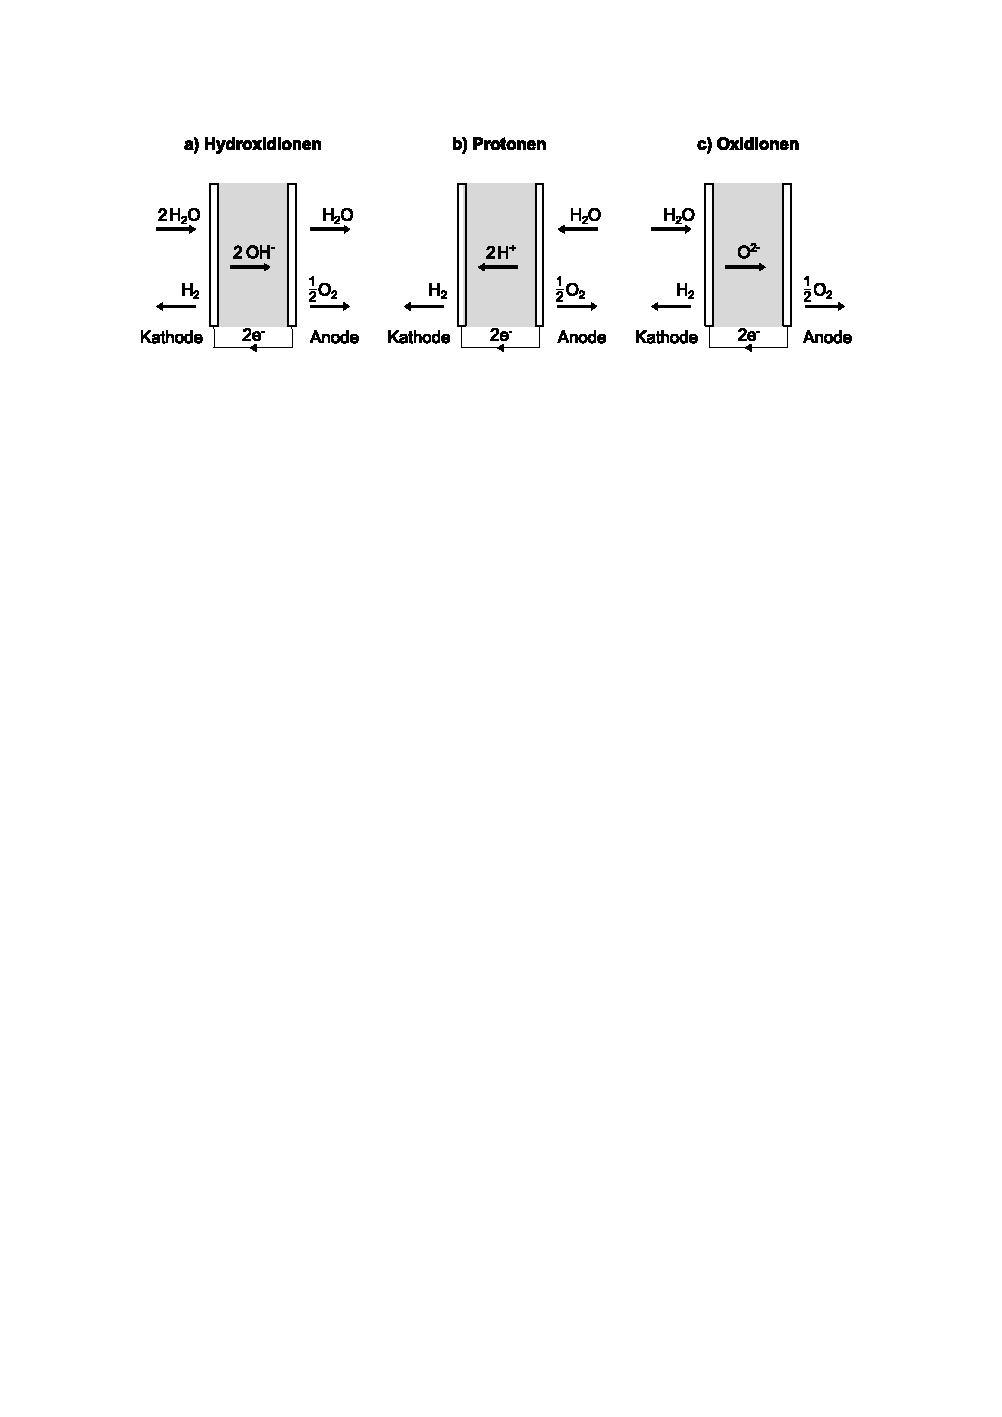
\includegraphics[scale=1]{Figures/LadungstraegerBeiDerWasserelektrolyse}
		\caption{Ladungsträger bei der 
		Wasserelektrolyse nach \citet{tjarks_pem-elektrolyse-systeme_2017}.}
\label{fig:LadungstraegerBeiDerWasserelektrolyse}	
\end{figure}

\subsection{Elektrochemische Betrachtung}
\label{subsec:Elektrochemische Betrachtung}
Die benötigte Energie bei einer Redoxreaktion entspricht der Reaktionsenthalpie $\Delta_R H$ und lässt sich aus den Bildungsenthalpien ($\Delta_f H_i$) und stöchiometrischen Koeffizienten ($\nu_i$) der Edukte und Produkte bestimmen \citep{falcao_review_2020,brauns_alkaline_2020}:
\begin{align}
 	\Delta_R H = \sum{\nu_i \cdot \Delta_f H_i}
\end{align}
Unter der Annahme, dass die nötige thermische Energie vorliegt, entspricht die zur Reaktion benötigte elektrische Energie  der freien Reaktionsenthalpie $\Delta_R G$, welche sich über die Reaktionsentropie $\Delta_R S$ errechnen lässt \citep{falcao_review_2020,brauns_alkaline_2020}.
\begin{align}
	\Delta_R G = \Delta_R H - T \cdot \Delta_R S \\
 	\Delta _R S = \sum{\nu_i S_i}
\end{align}

Für die Wasserelektrolyse (\ref{gl:Reaktionsgleichung}) bei Standardbedingungen ($T_0 = \SI{25}{\degreeCelsius}$ und $p_0 = \SI{101,325}{\kilo\pascal}$) ergibt sich mit den Daten aus Tabelle \ref{tb:Stoffdaten} die Reaktionsenthalpie zu $\Delta H^0_R = \SI{285,25}{\kilo\J\per\mol}$ und die freie Enthalpie zu $\Delta G^0_R = \SI{236,59}{\kilo\J\per\mol}$. Es liegt dabei eine starke Temperaturabhängigkeit vor, was in Abbildung \ref{fig:Entropien} deutlich wird.

\begin{table}[ht]
		\centering
		\caption{Standardbildungsenthalpien und Standardentropien für $\SI{25}{\degreeCelsius}$ \citep{koj_entwicklung_2021} sowie stöchiometrische Koeffizienten aus Gleichung \ref{gl:Reaktionsgleichung}.}
		
\begin{tabular}{c c c c}
		\toprule
		\multirow{2}{*}{Komponenten i} & 
		\multicolumn{1}{c}{$\Delta_f H^0_i$} & 
		
		\multicolumn{1}{c}{$S^0_i$} &
		
		\multicolumn{1}{c}{$\nu_i$}
		\\
		& 
		\multicolumn{1}{c}{$\textrm{[kJ/mol]}$}& 
		
		\multicolumn{1}{c}{$\textrm{[J/(molK)]}$} &
		\multicolumn{1}{c}{$\textrm{[---]}$}
		\\
		\midrule
		$\ce{H2O}$ & -285,25 & -216.35 &  -1\\
		$\ce{O2}$ & 0 &  21,78 &  $\textrm{1/2}$\\
		$\ce{H2}$ & 0 &  19,88 &  1\\
		\bottomrule
		\end{tabular}
		\label{tb:Stoffdaten}
		\end{table}	
			
\paragraph{Reversible Zellspannung}
\label{par:rev Zellspannung}
Mit der Faraday Konstante ($F=\SI{96485,3}{\coulomb\per\mol}$) und der Anzahl der pro Reaktion transferierten Elektronen ($z = 2$) lässt sich die thermoneutrale Spannung bei Standardbedingungen $U^0_{tn}$ sowie die reversible Zellspannung bei Standardbedingungen $U^0_{rev}$ errechnen \citep{falcao_review_2020}. 

\begin{align}
 U^0_{tn} = \frac{\Delta H^0_R}{zF} = \SI{1,478}{\volt}\\
 U^0_{rev} = \frac{\Delta G^0_R}{zF} = \SI{1,226}{\volt}
\end{align}

Der im vorherigen Abschnitt erläuterte Temperatureinfluss auf die Reaktionsbedingungen wirkt sich auch auf die reversible und thermoneutrale Spannungen aus (Abbildung \ref{fig:Entropien}). Häufig wird dieser Zusammenhang durch Gleichung \ref{gl:dT} abgebildet \citep{olivier_low-temperature_2017}.
Weiterhin liegt für die Zellspannung eine Abhängigkeit von den Produkt- und Edukt Aktivitäten vor, welche durch die Nernst Gleichung beschrieben werden kann. Drückt man die Aktivität der Produktgase über das Verhältnis des Partialdrucks zum Standarddruck $p_0$ aus, ergibt sich der in Gleichung \ref{gl:dp} angeführte Zusammenhang.\\

\begin{align}
U_{rev} = U^0_{rev} + \Delta U_{rev}(p) + \Delta U_{rev}(T)
\label{gl:Urev}\\
\Delta U_{rev}(T) = - 8,5 \cdot 10^{-4} \cdot (T-298)
\label{gl:dT}\\ 
\Delta U_{rev}(p) = \frac{RT}{zF}\ln{ \Bigl( \frac{p_{H_2}/p_0 \sqrt{p_{O_2}/p_0}}{a_{H_{2}O}}  \Bigr) } 	
\label{gl:dp}
\end{align} 

\begin{figure}[h]
	\centering
		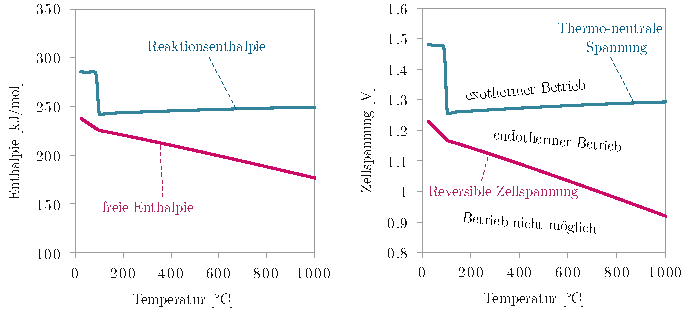
\includegraphics[scale=1]{Figures/VerlaufVonEntropien}
		\caption{Abhängigkeit der Reaktionsenthalpie und der freien Enthalpie von der Temperatur nach \citet{tremel_electrolysisfundamental_2018}.}
\label{fig:Entropien}	
\end{figure}

\subsubsection{Überspannungen}
\label{subsubsec:Überspannungen}
Die reale Zellspannung $U_{real}$ ist im Betrieb aufgrund von Verlusten immer größer als die reversiblen Zellspannung. Ist die reale Zellspannung niedriger, als die thermoneutrale Spannung, läuft das System endotherm ab. In dem Fall muss dem System Wärmeenergie zugeführt werden.\\
Als maßgeblichen Verluste, auch Überspannungen genannt, werden üblicherweise drei Phänomene betrachtet: Aktivierungsverluste ($U_{Akt}$), Ohmsche Verluste ($U_{Ohm}$) und Konzentrationsüberspannung \citep{falcao_review_2020}. In dieser Arbeit werden die Konzentrationsüberspannungen als vernachlässigbar klein angenommen, da sie erst außerhalb der üblichen Betriebsgrenzen von signifikanter Größenordnung sind. Ein weiteres Phänomen sind Diffusionsströme von Wasserstoff auf die Anodenseite und von Sauerstoff auf die Kathodenseite, allerdings sind diese aus Sicherheitsaspekten gering zu halten, was in \ref{subsec:Polarisationskurve} näher erläutert wird. Daher werden Diffusionsströme in dieser Arbeit vernachlässigt. Somit wird die reale Zellspannung wie folgt berechnet:\\

\begin{align}
	\label{gl:U_realEL}
	U_{real} =  U_{rev} + U_{Akt} + U_{Ohm}
\end{align}   

\paragraph{Aktivierungsverluste} kommen durch die elektrochemischen Vorgänge an den Oberflächen er Elektroden und ihrer Kinetik zustande. Dabei treten zwei Phänomene auf:  Einerseits chemische (wegen des chemischen Gleichgewichtszustands der Ionen an der Grenzfläche zwischen Elektrode und Elektrolyt) und andererseits elektrische (aufgrund des Ladungstransports durch das elektrische Feld an der Grenzfläche) \citep{stempien_solid_2013}. Aktivierungsverluste lassen sich mithilfe der Butler-Volmer-Gleichung beschreiben \citep{olivier_low-temperature_2017,stempien_solid_2013}. Zur Modellierung kann für ausreichend hohe Stromdichten vereinfachend die Tafel- Gleichung angewendet werden, \citet{abdin_modelling_2015} nutzen sie in der folgenden Form:\\

\begin{align}
	U_{Akt} = \frac{RT}{ 2 \cdot \alpha
		\cdot F} \cdot ln(i/i_0)
\label{gl:Akt}
\end{align}

Der Durchtrittsfaktor $\alpha$ und die Austauschstromdichte $i_0$ sind dabei experimentell zu ermitteln und unterscheiden sich je nach Bauart.\\

\paragraph{Ohmsche Verluste} werden durch elektrische sowie ionische Widerstände und Kontaktwiderständen zwischen den Komponenten verursacht. Ionischen Widerstände, welche sich in dem Elektrolyt  und an den Elektrodenoberflächen lokalisieren lassen, dominieren üblicherweise die Ohmschen Verluste \citep{stempien_solid_2013,milewski_modeling_2014}. Elektrisch Widerstände treten in den Elektroden und an den Kontakten der Zelle auf und lassen sich somit durch einen günstigen Aufbau der Zelle vermindern \citep{tjarks_pem-elektrolyse-systeme_2017}. Die ohmschen Verluste können mithilfe des Ohmschen-Gesetztes (Gleichung \ref{gl:Ohm}) bestimmt werden, für welches neben dem Elektrodenabstand auch die Leitfähigkeit des Elektrolyts benötigt wird.\\ 
\citet{olivier_low-temperature_2017} geben eine Gleichung zur Berechnung der Leitfähigkeit alkalischer Zellen an, dabei sind die Einflussfaktoren die Betriebstemperatur ($T$) sowie die Stoffmengenkonzentration ($m$) der Lauge des Elektrolyts. Die Berechnung der Leitfähigkeit für Festoxid (SO) Zellen ist \citet{hajimolana_mathematical_2011} entnommen. 
Der Ansatz für PEM-Zellen wird in der Literatur häufig verwendet \citep{falcao_review_2020, olivier_low-temperature_2017} und beachtet neben der Betriebstemperatur ($T$) auch den Feuchtegehalt der Membran ($\lambda$). \citet{tjarks_pem-elektrolyse-systeme_2017}  erweitert die Berechnung des ohmschen Wiederstandes nach Gleichung \ref{gl:Ohm2} um einen Parameter zur Berücksichtigung elektrische Widerstände $R_{el}$.

\begin{align}
	U_{Ohm} = &i \cdot (\delta / \sigma)
\label{gl:Ohm}\\
	U_{Ohm,PEM} = &  i \cdot (\delta / \sigma + R_{el})
\label{gl:Ohm2}
\end{align} \begin{align}
	\sigma _{Alk} = &   -2.04m -0.0028m^2  + 0.005332mT  \notag\\
				&+207.2m/T +0.001043m^3-3 \cdot 10^{-3}m^2T^2\\[2pt]
	\sigma _{SO} = &  3.34 \cdot 10^4 + exp(-10300/T)\\
	\sigma _{PEM} = &  (0.005139 \cdot \lambda -0.00326) \cdot \exp(1268 \cdot (1/303-1/T))
\end{align}

\subsection{Thermisches Verhalten}
\label{subsec:Thermisches Verhalten}
Zur Bestimmung des Wärmeflusses wird nach \citet{webster_implementation_2019} die Energiebilanz einer Elektrolysezelle betrachtet: 

\begin{align}
	C_{Zelle} \frac{\mathrm{d}T}{\mathrm{d}t} = \dot{n} (h_{ein} - h_{aus}) + P_{el} - \dot{Q} 
\end{align} 

Die Enthalpiedifferenz ergibt sich aus der Reaktionsenthalpie und der Temperaturdifferenz zwischen Eingang und Ausgang. Die benötigte Reaktionsenthalpie und die elektrische Leistung drückt \citet{webster_implementation_2019}	über die Thermoneutrale Spannung und die Zellspannung aus. Unter der Annahme, dass die   Ausgangstemperatur der Gase gleich der Betriebstemperatur ist, ergibt sich für die Energiebilanz damit:  
 
\begin{align}
	C_{Zelle} \frac{\mathrm{d}T}{\mathrm{d}t} = &-(\dot{n}_{H2, ein} \cdot c_{p, H2} +\dot{n}_{H2, ein} \cdot c_{p, O2}) \cdot (T_{ein} - T) \notag\\
	 &- I \cdot (U_{Zell} - U_{tn}) - \dot{Q}
	\label{gl:Energiebilanz}
\end{align}

\subsection{Polarisationskurve und Betriebsbereiche von Elektrolyseuren}
\label{subsec:Polarisationskurve}
Die Polarisationskurve gibt die Abhängigkeit der realen Zellspannung $U_{real}$ eines Elektrolyseurs von der Stromdichte graphisch wieder.  Diese wird von vielen Faktoren, wie beispielsweise den Elektrodenmaterialien, der Geometrie der einzelnen Bauteile oder den Betriebsbedingungen wie Druck und Temperatur, beeinflusst. Grundlage für die Berechnung der Polarisationskurve ist die in \ref{par:rev Zellspannung} hergeleitete reversible Zellspannung und Gleichung \ref{gl:U_realEL}. In Abbildung \ref{fig:PolarisationskurveElektrolyseure} werden die Polarisationskurven der in \ref{subsec:Technologien der Wasserelektrolyse} erläuterten technischen Verfahren verglichen.\\
\begin{figure}[h]
	\centering
		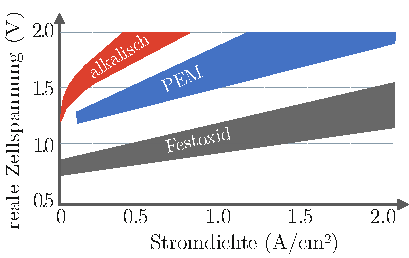
\includegraphics[scale=1]{Figures/PolarisationskurvenElektrolyseure}
		\caption{Mögliche Bereiche der Polarisationskurven der in \ref{subsec:Technologien der Wasserelektrolyse} erläuterten technischen Verfahren nach \citet{tremel_electrolysisfundamental_2018}.}
\label{fig:PolarisationskurveElektrolyseure}	
\end{figure}

Des weiteren lässt sich die Polarisationskurve auch zur Identifikation sinnvoller Betriebsbereiche nutzen:\\
Die elektrische Leistung einer Zelle ($P_{el}$) lässt sich aus der Stromdichte ($i$), der aktiven Fläche ($A_{zelle}$) und der realen Zellspannung errechnen. Das Faradaysche Gesetz liefert einen direkten Zusammenhang zwischen dem Elektronenfluss und dem Stoffmengenstrom des produzierten Wasserstoffs ($\dot{n}_{H_2O}$).
\begin{align}
	P_{el}(i) = &U_{real}(i)\cdot i A_{zelle}\\
	\dot{n}_{H_2O} = &\frac{i A_{zelle}}{zF}
	\label{gl:n_i}
\end{align}
Der Wirkungsgrad ($\eta$) einer Zelle, bezogen auf den unteren Heizwert ($H_u$) von Wasserstoff wird damit durch folgenden Ausdruck beschrieben:
\begin{align}
	\eta = \frac{H_u \cdot\dot{n}_{H_2O}}{P_{el}} = \frac{H_u}{U_{real}(i)\cdot{zF}}
\end{align}
Somit zeigt sich, dass es zur Steigerung der Effizienz erstrebenswert ist, den Elektrolyseur bei einer niedrigen Spannungen zu betreiben \citep{biaku_semiempirical_2008}. Aus Abbildung \ref{fig:PolarisationskurveElektrolyseure} wird ersichtlich, dass dies bei einer niedrigen Stromdichte der Fall ist. Allerdings bleibt zu bedenken, dass dadurch auch der Produktgas Strom verringert wird. Daher ist bei der Auslegung ein Kompromiss zwischen Wirkungsgrad und einer größeren aktive Zellfläche - und damit verbunden höheren Investitionskosten und größerem Bauraum - zu finden.\\
Weiterhin stellt die Gasreinheit der Produktströme eine untere Betriebsgrenze für die Stromdichte dar. Aufgrund der Diffusion der Produktgase zur gegenüberliegenden Elektrode kommt es zu einer Mischung von Sauerstoff und Wasserstoff. Um die Zerstörung des Systems durch Explosionen zu verhindern, geben \citet{brauns_alkaline_2020} an, dass meist bei einer Verunreinigung über 2 Volumen-\%  ein Notstopp des gesamten Elektrolyseur-Systems eingeleitet wird. Daher werden Grenzwerte für den maximalen Betriebsdruck und die minimale Stromdichte empfohlen, weil diese beiden Größen die Gasreinheit signifikant beeinflussen.\\

\subsection{Technologien der Wasserelektrolyse}
\label{subsec:Technologien der Wasserelektrolyse}
Im Folgenden werden die drei maßgeblichen Verfahren zur Wasserelektrolyse näher erläutert und verglichen.
\paragraph{Alkalischer Elektrolyseur}
\label{par:Alkalischer Elektrolyseur}
Die alkalische Elektrolyse ist eine ausgereifte Technik und der derzeitige Standard für groß dimensionierte Elektrolyseure \citep{tremel_electrolysisfundamental_2018}. Anlagen mit einer Eingangsleistung von bis zu \SI{130}{\mega\W}  sind derzeit im Betrieb und die minimale Teillast liegt nach \citet{guandalini_comparative_2016} bei ungefähr $\SI{20}{\%}$. Als Elektrolyt dient üblicherweise zwischen 25 und 30 prozentige Natron- (NaOH) oder Kalilauge (KOH) \citep{tremel_electrolysisfundamental_2018}. Die Konzentration beeinflusst dabei maßgeblich die Leitfähigkeit der Lösung. Als Ladungsträger in der Lösung fungieren Hydroxidionen. Es werden metallische Elektroden verwendet, welche zur Steigerung der Aktivität mit Edelmetallen beschichtet werden können. Folgende Reaktionen laufen an der Kathode und Anode ab:
\begin{align}
  \ce{	&{Kathode:} &2H2O + 2 e^- &-> H2 + 2OH^-\\
  		&{Anode:} &2OH^- &-> H2O + O2 + 2 e^-} 
\end{align}
Um die produzierten Gase voneinander getrennt zu halten, wird zwischen Anode und Kathode ein Diaphragma positioniert. Dies hat neben Performance- auch Sicherheitsgründe, da elementarer Wasserstoff hochentzündlich ist. Aus diesem Grund sind Elektrolyseure auch in ihrer Dynamik eingeschränkt: Bevor das System abgeschaltet werden kann, müssen die Gasleitungen mit Inertgas gefüllt werden, um die Bildung einer explosiven Wasserstoff-Sauerstoff Mischung zu verhindern. Dies hat auch einen Einfluss auf den Anlaufvorgang des Systems, da die Gasqualität durch die anfangs vorliegenden Inertgase vermindert wird. Nach \citet{milanzi_technischer_2018} kann das dynamische Verhalten von Elektrolyseuren erheblich verbessert werden, wenn sie während Standzeiten im Standby betrieben werden. \\ 
Ein weiterer Nachteil aktueller technischer Anlagen der alkalischen Elektrolyse ist, dass die maximale Stromdichte verglichen mit anderen Elektrolyseuren niedrig ausfällt (\citet{tremel_electrolysisfundamental_2018} gibt Stromdichten von $0,2-\SI{0,5}{\A\per\cm\squared}$ an).

\paragraph{Protonen Austausch Membran (PEM) Elektrolyseur}
\label{par:Protonen Austausch Membran (PEM) Elektrolyseur}
PEM-Elektrolyseure werden seit 1950 entwickelt und derzeit im $\SI{1}{\mega\W}$ Bereich vertrieben. Ein Vorteil der Technologie sind die hohen erreichbaren Stromdichten von bis zu $\SI{2}{\A\per\cm\squared}$. Zudem können PEM-Elektrolyseure sehr dynamisch betrieben werden und ein Betrieb bei bis zu 10\% minimaler Teillast ist möglich \citep{tremel_electrolysisfundamental_2018}.\\
Als Ladungsträger fungieren Protonen und als Elektrolyt dient eine in destilliertem Wasser positionierte Protonen-Austausch-Membran (\textbf{P}roton \textbf{E}xchange \textbf{M}embran).
Die Protonenleitfähigkeit der Polymer-Membran wird durch Sulfonsäure-bindende Seitengruppen, sogenannte Idomere, erreicht \citep{tjarks_pem-elektrolyse-systeme_2017}.  Für die Dicke der Membran muss dabei ein Kompromiss zwischen Langlebigkeit und Durchlässigkeit gefunden werden \citep{falcao_review_2020}. Der Säuregehalt des Elektrolyts und die damit verbundene Anforderung an die Korrosionsbeständigkeit, so wie das Erstreben hoher Reaktionsgeschwindigkeiten führt zu hohen Kosten bei den Elektrodenmaterialien: Die Kathode besteht meist aus mit Platin beschichtetem Kohlenstoff, als Anode werden häufig als Oxid vorliegendes Irdium oder Ruthenium verwendet. Folgende Reaktionen laufen an der Kathode und Anode ab:
\begin{align}
  \ce{	&{Kathode:} &2H^+ + 2e^- &-> H2\\
  		&{Anode:} &H2O  &->  1/2O2 + 2H^+ + 2 e^-}
\end{align}
  		
\paragraph{Festoxid-Elektrolyseur}
\label{par:Festoxid-Elektrolyseur}
Feststoffoxid(SO) Elektrolyseure sind seit 1980 in Entwicklung \citep{tremel_electrolysisfundamental_2018}. Sie haben  den Vorteil, dass sie bei Temperaturen von $700-\SI{1000}{\degreeCelsius}$ betrieben werden, wodurch dampfförmiges Wasser zerlegt wird, wohingegen bei alkalischen und PEM-Elektrolyseuren flüssiges Wasser vorliegt. Daraus resultiert, dass Reaktionsenthalpie und dadurch auch die reale Zellspannung niedriger ausfällt. Dieser Effekt wird dadurch verstärkt, dass bei hohen Temperaturen die ohmschen Verluste sinken, wodurch niedrigere Überspannungen entstehen \citep{tremel_electrolysisfundamental_2018}. Zudem steigt mit der Temperatur auch die Reaktionsgeschwindigkeit, weshalb keine teuren Katalysator-Materialien verwendet werden müssen \citep{yan_performance_2017}.\\
Ein Nachteil der gesteigerten Betriebstemperatur sind die höheren Ansprüche an die Temperaturbeständigkeit der Elektroden und des Elektrolyts. Als Elektrolyt wird meist Zirkoniumdioxid ($\ce{ZrO2}$) verwendet, welches zur Steigerung der Leitfähigkeit mit Yttriumoxid ($\ce{Y2O3}$) stabilisiert wird \citep{butz_decomposition_2009}.
Das Elektrolyt wird zwischen zwei porösen Elektroden (Beispielsweise eine Nickeloxid Anode und eine LSCF-Kathode \citep{schiller_high_2010}) positioniert, was den Austausch der Oxidionen ermöglicht. Es existieren SO-Elektrolyseure, welche auf dem Transport von Protonen basieren, allerdings wird aufgrund ihrer geringen Bedeutung  in dieser Arbeit nicht weiter darauf eingegangen \citep{stempien_solid_2013}. Folgende Reaktionsgleichungen liegen bei den betrachteten Festoxid-Elektrolyseuren vor:
\begin{align}
  \ce{	&{Kathode:} &H2O &-> H2 + O^2- + 2e^-\\
  		&{Anode:} &O^2- + 2 e^-  &->  1/2O2} 
\end{align}
Eine Herausforderung ist das Bereitstellen der benötigten Wärme zur Wasserdampferzeugung und zum Aufrechterhalten der Betriebstemperatur. Dazu werden verschiedene Möglichkeiten, wie beispielsweise die Kopplung mit Wärmepumpen oder Sonnenkollektoren in Betracht gezogen \citep{stempien_solid_2013}. Weiterhin bleibt ein zu lösendes Problem der Leistungsverlust und der Abbau der Elektrodenmaterialien, was die Lebensdauer der Zellen signifikant einschränkt \citep{yan_performance_2017}.\\

Abschließend sind in Tabelle \ref{tb:VglElektrolyseur} wichtige Kennwerte der drei Technologien sowie ihre Vor- und Nachteile aufgeführt.

\begin{table}[ht]
		\centering
		\caption{Vergleich der gängigen Technologien zur Wasserelektrolyse nach \citet{milanzi_technischer_2018}, \citet{tremel_electrolysisfundamental_2018} und \citet{rashid_hydrogen_2015}.}
		\begin{tabular}{l c c c}
		\toprule
		 & alkalisch & PEM & Festoxid
		\\
		\midrule
		Temperatur & $40 - \SI{90}{\degreeCelsius}$ & $20 - \SI{100}{\degreeCelsius}$ & $700-\SI{1000}{\degreeCelsius}$\\
		min. Teillast & 20\% & 10\% & 30\% \\
		max. Stromdichte & $0,2 - \SI{0,5}{\A\per\cm\squared}$ & $\SI{2}{\A\per\cm\squared}$ & $\SI{1}{\A\per\cm\squared}$\\
		max. Lastgradient & $\SI{33}{\%\per\s}$ & $\SI{100}{\%\per\s}$ & \\
		\midrule
		Vorteile & geringer Preis & Kompaktheit & Wirkungsgrad\\
		& Technologiereife & Betriebsbereich & günstiger Katalysator\\
		& Lebensdauer & Lastgradient & hoher Betriebsdruck\\
		& & Gasreinheit&\\
		\midrule
		Nachteile & geringe Gasreinheit & hohe Kosten & Technologiereife\\
		& korrosives Elektrolyt & saures Elektrolyt & Lebensdauer\\
		& geringer Betriebsdruck & lange Anfahrzeit & \\
		\bottomrule
		\end{tabular}
		\label{tb:VglElektrolyseur}
\end{table}	


\subsection{Grundlagen von Brennstoffzellen}
\label{subsec:BZ}
In Brennstoffzellen wird der Umkehrprozess der Elektrolyse betrieben. Die chemische Reaktionsenergie eines Kraftstoffes wird in elektrische Energie umgewandelt. Bei Wasserstoff betriebenen Brennstoffzellen läuft die Reaktion \ref{gl:Reaktionsgleichung} rückwärts ab, es wird aus Wasserstoff und Sauerstoff Wasser gebildet. Der Aufbau von Brennstoffzellen gleicht dem von Elektrolyseuren: Es werden zwei Elektroden, ein Elektrolyt sowie gegebenenfalls ein Diaphragma zur Gastrennung verwendet. Daher werden einige Zellen sowohl als Brennstoffzelle als auch als Elektrolyseur eingesetzt \citep{yan_performance_2017}. Ein Vorteil der Brennstoffzelle ist dabei, dass sowohl reiner Sauerstoff als auch Umgebungsluft zur Kombination mit Wasserstoff verwendet werden kann \citep{olabi_prospects_2020,jiao_challenges_2017}.\\
Die in \ref{subsec:Elektrochemische Betrachtung} genannten elektrochemischen Grundlagen lassen sich auf die Brennstoffzelle übertragen: Die reversible Zellspannung $U_{rev}$ entspricht der maximalen Ausgangsspannung der Brennstoffzelle. Weil $U_{rev} < U_{th}$ wird stets weniger elektrische Energie abgeführt, als chemische Energie zugeführt wird, es liegt also eine exotherme Reaktion vor. Da die in \ref{subsubsec:Überspannungen} beschriebenen Verlustmechanismen durch Diffusionsvorgänge und ohmsche Widerstände hervorgerufen werden, treten sie auch bei Brennstoffzellen auf \citep{chugh_experimental_2020}. Allerdings werden die Verlustterme von der reversiblen Zellspannung subtrahiert:\\
\begin{align}
	\label{gl:U_real-BZ}
	U_{real} =  U_{rev} - U_{Akt} - U_{Ohm} - U_{Diff}
\end{align}   

Wie auch bei Elektrolyseuren existieren für die Umsetzung von reinem Wasserstoff alkalische, PEM und Festoxid Brennstoffzellen \citep{lucia_overview_2014}. Auf weitere Technologien, welche Methan, Erdgas oder vergaste Kohle als Energieträger verwenden wird in dieser Arbeit nicht näher eingegangen.\\
Während die elektrochemischen Grundlagen der Brennstoffzelle bereits im 19. Jahrhundert entdeckt wurden, entwickelte die NASA   gegen Ende der 1950er die ersten alkalischen und PEM Brennstoffzellen für Raumfahrtanwendungen. Auffällig ist, dass im Gegensatz zur Elektrolyse, bei der heutzutage bei großen Anlagen alkalische Elektrolyseure der Stand der Technik sind (\ref{par:Alkalischer Elektrolyseur}), bei den Brennstoffzellen die PEM-Technologie deutlich verbreiteter ist. So gibt \citet{lucia_overview_2014} an, dass 2010  der Marktanteil der PEM-Technologie bei Brennstoffzellen bei 97\% lag. Eine mögliche Erklärung dafür ist, dass Brennstoffzellen vorwiegend bei mobilen Anwendungen eingesetzt werden - nach \citet{lucia_overview_2014} ist dies bei 95\% aller verkauften Brennstoffzellen der Fall. Die Vorteile von Brennstoffzellen sind dabei die geringen Geräusch- und Schadstoffemissionen \citep{olabi_prospects_2020}. Für mobile Anwendungen eignen sich insbesondere PEM-Brennstoffzellen, da diese bei einer höheren maximalen Stromdichte betrieben werden können als alkalische und Festoxid-Zellen. Das wiederum bringt  Vorteile im Bezug auf den benötigten Bauraum und das Gewicht mit sich.\\ 
Eine weiteres Anwendungsgebiet von Brennstoffzellen ist aufgrund des exothermen Betriebs die Kraft-Wärme-Kopplung. \citet{olabi_prospects_2020} geben an, dass Brennstoffzellen höhere Gesamt-Wirkungsgrade erreichen als andere klein-skalierte Systeme zur Kraft-Wärme-Kopplung. Dabei ist zu beachten, dass die Qualität der Abwärme insbesondere von der Betriebstemperatur der Brennstoffzelle abhängt, was nach Tabelle \ref{tb:VglBz} für den Einsatz von Festoxid-Brennstoffzellen spricht.\\ 
In Tabelle \ref{tb:VglBz} werden wichtige Kennwerte der drei Technologien sowie ihre Vor- und Nachteile angegeben.\\

\begin{table}[ht]
		\centering
		\caption{Vergleich der gängigen Technologien Wasserstoff-basierter Brennstoffzellen nach \citet{mekhilef_comparative_2012}.}
		\begin{tabular}{l c c c}
		\toprule
		 & alkalisch & PEM & Festoxid
		\\
		\midrule
		Temperatur & $90 - \SI{100}{\degreeCelsius}$ & $50 - \SI{100}{\degreeCelsius}$ & $600-\SI{1000}{\degreeCelsius}$\\
		el. Wirkungsgrad & 60\% & 53-58\% & 35-43\% \\
		ges. Wirkungsgrad & 80\% & 70-90\% & 80\%\\
		\midrule
		Vorteile & Preis & Kompaktheit & günstiger Katalysator\\
		& Technologiereife & Lebensdauer & Effizienz\\
		&  & kurze Anfahrzeit & \\
		\midrule
		Nachteile & Empfindlich bei $\ce{CO2}$ &  & Technologiereife\\
		& korrosives Elektrolyt & saures Elektrolyt & Lebensdauer\\
		& geringer Betriebsdruck & & lange Anfahrzeit\\
		\bottomrule
		\end{tabular}
		\label{tb:VglBz}
		\end{table}	
		
\subsection{Benötigte Systemkomponenten}
\label{subsec:Systemkomponenten}
Die zum Betrieb von Elektrolyseuren und Brennstoffzellen benötigt Komponenten werden in dem folgenden Abschnitt erläutert,  da sie einen wesentlichen Einfluss auf das Verhalten des Gesamtsystems haben. Abbildungen \ref{fig:ProzessElektrolyse} sowie \ref{fig:ProzessBrennstoffzelle} liefern dazu einen Überblick.

\begin{figure}[h]
	\centering
		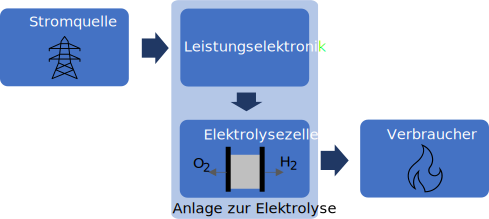
\includegraphics[scale=1]{Figures/ElektrolyseurProzessschritte}
		\caption{Übersicht der benötigten Systemkomponenten zum Betrieb eines Elektrolyseurs \citep{tjarks_pem-elektrolyse-systeme_2017}.}
\label{fig:ProzessElektrolyse}	
\end{figure}

\begin{figure}[h]
	\centering
		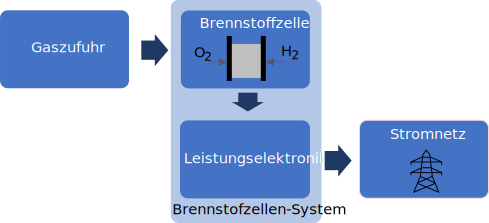
\includegraphics[scale=1]{Figures/BrennstoffzelleProzessschritte}
		\caption{Übersicht der benötigten Systemkomponenten zum Betrieb einer Brennstoffzelle.}
\label{fig:ProzessBrennstoffzelle}	
\end{figure}

Im Falle der Elektrolyse wird die Leistungselektronik benötigt, um zwei Aufgaben zu erfüllen:
Erstens die Anpassung der Versorgungsleistung auf die elektrischen Anforderungen des Elektrolyseurs und zweitens die Wandlung der Wechselspannung zu Gleichspannung \citep{tjarks_pem-elektrolyse-systeme_2017}.
Stand der Technik sind Thyristor-basierte Gleichrichter, welche sich durch geringe Verluste auszeichnen.
Als Nachteil dieser Technik ist allerdings zu nennen, dass die Schaltfrequenz an die Netzfrequenz gekoppelt ist, was die Restwelligkeit der Ausgangsgrößen erhöht.
Transistor-basierte Gleichrichter versprechen im Bereich der Restwelligkeit wesentliche Verbesserungen und durch aktuelle Entwicklungen konnten die auftretenden Schaltverluste  signifikant verringert werden \citep{tjarks_pem-elektrolyse-systeme_2017}.\\

Im Falle der Brennstoffzelle wird die Leistungselektronik benötigt, um die erzeugte Gleichspannung zu Wechselspannung zu transformieren und den elektrischen Anforderungen des Netzes anzupassen.
Nach \citet{engler_wechselrichter_nodate} haben sich im Bereich der Wechselrichter Transistor-basierte Systeme etabliert.
Häufig werden Niederfrequenz Transformatoren verwendet, welche sich durch eine hohe Zuverlässigkeit auszeichnen, allerdings Nachteile bei dem Gewicht und der Baugröße aufweisen.
Ein Entwicklungsfeld sind daher Hochfrequenztransformatoren, die ein geringeres Gewicht und einen kleineren Bauraum ermöglichen.
\chapter{Methode+Anwendung}
\label{cha:Methode+Anwendung}

\section{K.A.}
\label{sec:Sektion 1}

\subsection{Modell Aufbau}
\label{subsec:Abschnitt1}
In diesem Abschnitt sollen der Aufbau der Modelle erläutert werden.
\subsection{Modellgleichungen}
 Gleichungen 

\subsection{Szenarien Vorstellen}
LIYDNvkluksah.dygvÖSRi.ldgh.kvnr sd



\section{Blindtext}


\Blindtext %Command for generating text automatically

\chapter{Simulation der Systemkomponenten und Diskussion der Ergebnisse}
\label{cha:Diskussion}
Im folgenden Kapitel werden die Simulationsergebnisse vorgestellt. Zur Plausibilisierung der Daten werden die Modelle der Wasserstoffkomponenten im ersten Schritt mit in der Literatur angegebenen Messwerten abgeglichen. Im zweiten Schritt folgt die Präsentation der Simulationsergebnisse samt Berechnung der zur Bewertung herangezogenen Kennwerte. Dabei erfolgt zudem ein Vergleich der Systemkonzepte anhand der Bewertungskriterien.
 
\section{Validierung der Komponentenmodelle}
\label{sec:Sektion 1}
In der folgenden Validierung werden drei Systeme betrachtet: Einerseits ein alkalischer Elektrolyseur und eine PEM-Brennstoffzelle, weil diese beiden Bauarten in den Systemkonzepten genutzt werden. Andererseits ein PEM-Elektrolyseur, da diese Bauart, wie in \ref{subsec:Technologien der Wasserelektrolyse} angegeben, aufgrund von Vorteilen in der Dynamik der Last und bei der Baugröße aktuell an Relevanz zunehmen. 

\subsection{Komponenten der Systemkonzepte}
Zur Validierung des alkalischen Elektrolyseurs werden die von \citet{hammoudi_new_2012} dokumentierten Messwerte genutzt. Betrachtet wird eine Einzelzelle mit einer aktiven Zellfläche von $\SI{0,03}{\m\squared}$ deren Elektrodenabstand mit $\SI{5}{\milli\m}$ angenommen wird. Als Elektrolyt dient $30$-prozentige Kalilauge (daraus folgt $m=\SI{6,85}{\mol\per\l}$ \citep{periodensystem-online_dichtewerttabelle_nodate}). Betrieben wird die Zelle bei einem Druck von $\SI{1}{\bar}$ und es wird eine Temperatur von $30$ sowie $\SI{53,5}{\degreeCelsius}$ betrachtet.

\begin{figure}[h]
	\centering
		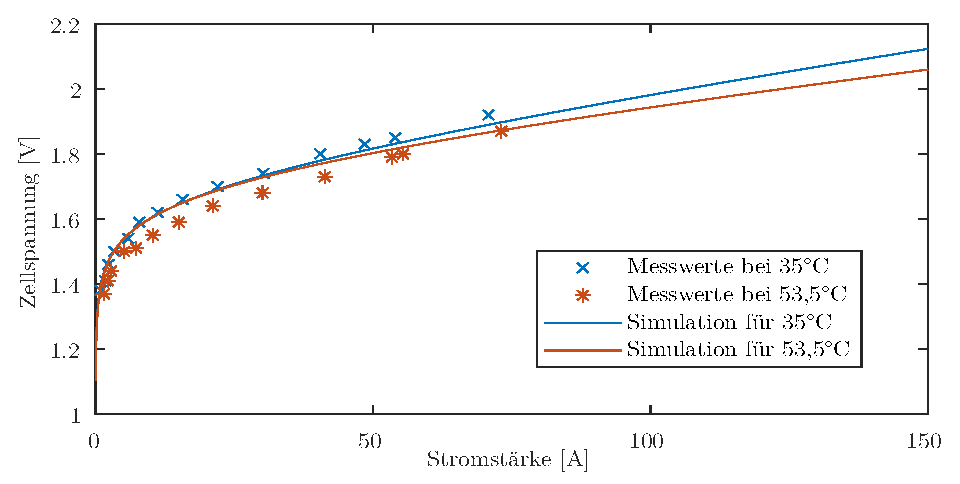
\includegraphics[scale=1]{Figures/ValidierungALK}
		\caption{Vergleich des Elektrolyseur-Modells mit Messwerten von \citet{hammoudi_new_2012}.}
\label{fig:ValALK}	
\end{figure}

Der von \citet{hammoudi_new_2012} dokumentierte Maximalwert der Stromstärke beträgt $\SI{73}{\A}$ und die minimale Teillast wird, wie in \ref{tb:VglElektrolyseur} angegeben, mit $\SI{20}{\%}$ des Maximalwerts angenommen. Somit kann als minimale Teillast des Elektrolyseurs im realen Betrieb von einer Stromstärke von $\SI{14,6}{\A}$ ausgegangen werden. In diesem Bereich beträgt der Fehler bei einer Temperatur von $\SI{35}{\degreeCelsius}$ maximal $\SI{1,6}{\%}$. Für eine Temperatur von $\SI{53,5}{\degreeCelsius}$ ergibt sich eine maximale Abweichung von $\SI{3,5}{\%}$ (Im Durchschnitt $\SI{2,2}{\%}$).\\
Es zeigt sich also, dass das Modell in der Lage ist, die Polarisationskurven alkalischer Elektrolyseure mit hinreichender Genauigkeit zu modellieren. Somit ist es für die Anwendung im Rahmen dieser Arbeit geeignet. Für folgende Arbeiten wird eine Validierung des Modells bei verschiedenen Druckniveaus empfohlen.\\

Um die Rechenzeit der Simulation gering zu halten wird in dieser Arbeit auf eine Simulation des thermischen Verhaltens der Elektrolysezelle verzichtet, allerdings kann diese bei Bedarf ohne weiteren Entwicklungsaufwand aus dem Brennstoffzellenmodell übernommen werden.
Eine weitere Möglichkeit zur Ausweitung des Modells sind dynamische Vorgänge, die in dieser Arbeit aufgrund der großen Zeitschritte der Simulation nicht beachtet wurden (Ausführlichere Begründung in \ref{subsec:Modellierung der Zelle}). Um diese zu berücksichtigen, kann die in der Energiebilanz (Gleichung \ref{gl:Energiebilanz}) enthaltene Instationarität der Zelltemperatur in der Modellierung des thermischen Verhaltens übernommen werden.\\

Zur Validierung der PEM-Brennstoffzelle werden Messwerte von \citet{chugh_experimental_2020} genutzt. Es handelt sich um einen Brennstoffzellenstack von 30 in Reihe geschalteten Einzelzellen. Die aktive Zellfläche einer Einzelzelle beträgt $\SI{0,005}{\m\squared}$ und die Dicke der Membran ist mit $\SI{50,8}{\micro\m}$ angegeben. Die betrachtete Betriebstemperatur beträgt $50$ und $\SI{80}{\degreeCelsius}$ und der Betriebsdruck bei $1$ und $\SI{2,5}{\bar}$.

\begin{figure}[h]
	\centering
		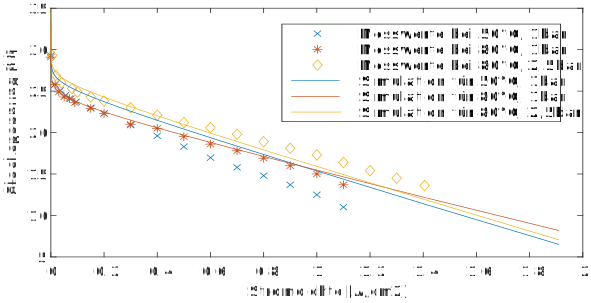
\includegraphics[scale=1]{Figures/ValidierungPEMFC}
		\caption{Vergleich des Brennstoffzellen-Modells mit Messwerten von \citet{chugh_experimental_2020}.}
\label{fig:ValPEMFC}	
\end{figure}

\citet{chugh_experimental_2020} dokumentieren einen Stromstärke von bis zu $\SI{1,4}{\A\per\cm\squared}$ und die minimale Teillast wird, wie in \ref{tb:VglBz} angegeben, für PEM-Zellen mit $\SI{10}{\%}$ des Maximalwerts angenommen. Daraus ergibt sich eine minimale Teillast von $\SI{0,14}{\A\per\cm\squared}$ für den realen Betrieb. Oberhalb des genannten Wertes liegt der Fehler bei einer Temperatur von $\SI{50}{\degreeCelsius}$ und einem Druck von $\SI{1}{\bar}$ zwischen $6,2$ und $\SI{30,6}{\%}$. Für $\SI{80}{\degreeCelsius}$ und $\SI{1}{\bar}$ ergeben sich Abweichungen von durchschnittlich $\SI{2,1}{\%}$ (Die maximale Abweichung beträgt $\SI{7,6}{\%}$). Wird der Druck auf $\SI{2,5}{\bar}$ angehoben, steigt der Fehler auf durchschnittlich $\SI{5,3}{\%}$ (Die maximale Abweichung beträgt in dem Fall $\SI{11,1}{\%}$).\\

Es zeigt sich somit, dass das Modell die Polarisationskurve von Brennstoffzellen bei hohen Betriebstemperaturen in einem akzeptablen Maß approximiert. Da die zur Simulation der Systemkonzepte eingesetzte Brennstoffzelle bei einer Betriebstemperatur von $\SI{80}{\degreeCelsius}$ betrieben wird, ist im Bezug auf die Modellierung der Brennstoffzelle von einer ausreichenden Genauigkeit auszugehen.\\
Die großen Abweichungen bei niedrigen Temperaturen lassen sich durch die Wahl des Durchtrittsfaktors ($\alpha$) und der Austauschstromdichte ($i_0$) begründen. Wie von \citet{falcao_review_2020} gezeigt, variieren die in der Literatur angegebenen Werte der beiden Parameter stark. So liegen die Angaben des Durchtrittfaktors zwischen $2$ und $0,5$ - die Angaben der Austauschstromdichte schwanken von $\SI{e-3}{}$ bis $\SI{e-9}{\A\per\cm\squared}$. Dabei werden teilweise getrennte Werte für Anode und Kathode angegeben, was aber auf die Größenordnung des Wertebereichs keinen Einfluss nimmt (Die angegebenen Wertebereiche beziehen sich auf die Anode, da dort höhere Verluste auftreten).\\
Es wird ersichtlich, dass die experimentell ermittelten Parameter einerseits von dem Aufbau des Modells abhängen, denn die Fitting-Parameter werden sowohl durch die Modellierung der anderen Verluste als auch durch im Modell nicht berücksichtigte weitere Faktoren beeinflusst. Andererseits spielt der Versuchsaufbau und die untersuchte Zelle eine gewichtige Rolle, da beispielsweise die Betriebstemperatur, der Betriebsdruck oder Materialeigenschaften die resultierenden Fitting-Parameter beeinflussen.
Einige Autoren nutzten daher Approximationen, um einen Temperatureinfluss auf den Durchtrittsfaktor oder die Austauschstromdichte im Modell zu berücksichtigen \citep{falcao_review_2020,milewski_modeling_2014}. Für die Modellierung von PEM-Zellen verspricht dies eine 
Steigerung der Genauigkeit bei niedrigen Temperaturen. Ob diese Maßnahme die Genauigkeit der Modellierung von alkalischen Zellen erhöht ist unklar, da die Validierungsergebnisse des alkalischen Elektrolyseurs keine signifikante Steigerung der Abweichungen bei zu- oder abnehmenden Temperaturen dokumentieren.\\
Eine weitere Möglichkeit zur Steigerung der Genauigkeit bei der Modellierung der Brennstoffzelle könnte die Beachtung der Konzentrationsüberspannungen sein. Denn diese treten insbesondere im oberen Lastbereich auf, und in diesem sind bei der Validierung zunehmende Abweichungen zu erkennen.\\

Die Validierung der Systemkomponenten ist somit im Hinblick auf die Genauigkeit der Simulationsergebnisse insgesamt als positiv zu bewerten: Die Elektrolysezelle wird über den abgebildeten Bereich zufriedenstellend modelliert. In dem für die Simulation relevanten Betriebspunkt trifft dies auch auf die Modellierung der PEM-Brennstoffzelle zu. Somit sind die in \ref{sec:Ergebnisse} präsentierten Simulationsergebnisse zur vorläufigen Bewertung der Systemkonzepte geeignet.
In Zukunft sollte darüber hinaus eine Validierung der Modellierung des thermischen Verhaltens erfolgen.

\subsection{PEM-Elektrolyseur}
Die Daten zur Validierung der PEM-Elektrolysezelle sind \citet[S. 36]{tjarks_pem-elektrolyse-systeme_2017} entnommen. Betrachtet wird eine Einzelzelle mit einer aktiven Zellfläche von $\SI{0,0025}{\m\squared}$ deren Membran mit einer Dicke von $\SI{150}{\micro\m}$ abgeschätzt wird (vergleiche \citet{rashid_hydrogen_2015}).
Es werden Betriebstemperaturen von $30$, $60$ und $\SI{80}{\degreeCelsius}$ bei einem Druck von $\SI{1}{\bar}$ untersucht.\\

\begin{figure}[h]
	\centering
		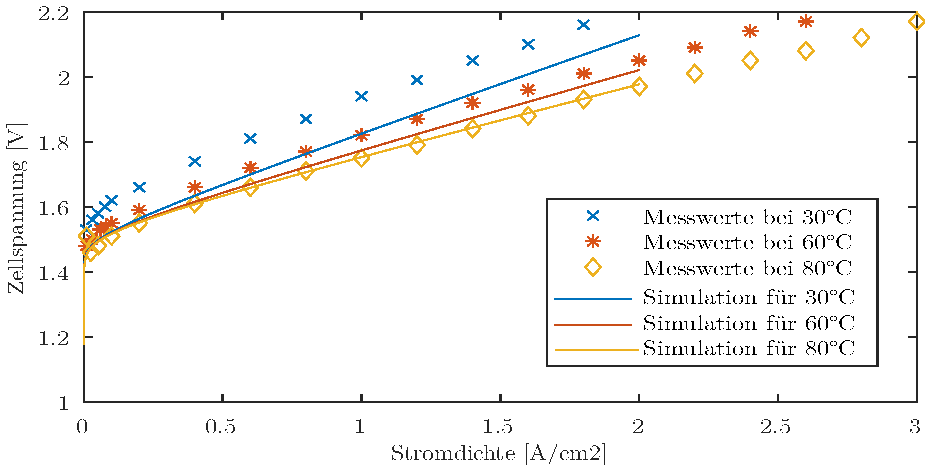
\includegraphics[scale=1]{Figures/ValidierungPEMEC}
		\caption{Vergleich des Elektrolyseur-Modells mit Messwerten von \citet{tjarks_pem-elektrolyse-systeme_2017}.}
\label{fig:ValPEMEC}	
\end{figure}

Die folgenden Angaben beziehen sich auf Stromdichten oberhalb von $\SI{0,2}{\A\per\cm\squared}$, da die minimale Teillast nach Tabelle \ref{tb:VglBz} für PEM-Zellen mit $\SI{10}{\%}$ der Maximalen Stromdichte angenommen wird. Bei einer Temperatur von $\SI{30}{\degreeCelsius}$ ergeben sich Abweichungen von  $\SI{22,3}{\%}$ bei der minimalen Teillast und $\SI{4,4}{\%}$ bei Maximallast. 
Für eine Temperatur von  $\SI{60}{\degreeCelsius}$ liegt der Fehler über den gesamten Leistungsbereich unter $\SI{2,9}{\%}$, für $\SI{80}{\degreeCelsius}$ unterhalb von $\SI{0,5}{\%}$.\\

Es zeigt sich somit auch für den PEM-Elektrolyseur, dass das Modell im oberen Temperaturbereich in der Lage ist, die Polarisationskurve ausreichend genau abzubilden. Wie auch bei der PEM-Brennstoffzelle liegen bei niedrigen Temperaturen signifikante Abweichungen zu den Messwerten vor. Im Gegensatz zur Brennstoffzelle nehmen diese aber nicht bei hohen, sondern bei niedrigen Lasten zu. Außerdem zeigt ein Vergleich der Messwerte des PEM-Elektrolyseurs und der PEM-Brennstoffzelle, dass sich der Temperatureinfluss auf die Zellspannung in den beiden Fällen deutlich unterscheidet:\\ 
Im Falle der Brennstoffzelle (Abbildung \ref{fig:ValPEMFC}) zeigt sich eine gesteigerte Temperatur erst im oberen Lastbereich, wohingegen sich die Zellspannung bei $0,2$ bis $\SI{0,3}{\A\per\cm\squared}$ trotz einen Temperaturdifferenz von $\SI{30}{\degreeCelsius}$ nicht signifikant unterscheidet.\\
Im Falle des Elektrolyseurs (Abbildung \ref{fig:ValPEMEC}) ist schon im unteren Lastbereich ein signifikanter Unterschied der Zellspannung für die abgebildeten Temperaturen sichtbar, der mit zunehmender Stromdichte linear ansteigt.\\

Daraus lässt sich schlussfolgern, dass für den gewählten Elektrolyseur und die Brennstoffzelle eine einheitliche Parametrierung insbesondere über einen größeren Temperaturbereich keine zufriedenstellenden Ergebnisse liefern kann. Ob diese Beobachtung allgemein auf den Vergleich von Elektrolyseuren und Brennstoffzellen anzuwenden ist, bleibt allerdings unklar. In folgenden Arbeiten sollte daher untersucht werden, ob weitere Messreihen den unterschiedlichen Temperatureinfluss auf die Polarisationskurven bestätigen. Dies würde im Modell gegebenenfalls eine getrennte Parametrierung von Brennstoffzellen und Elektrolyseuren erfordern.\\

\section{Ergebnisse der Simulationen der Systemkonzepte}
\label{sec:Ergebnisse}
Die Simulationen wurden mit Zeitschritten von $\SI{900}{\s}$ ($=\SI{15}{\minute}$) durchgeführt. Es wurde der Dymola-Standard-Löser \textit{Dassl} mit einer Toleranz von $\SI{e-4}{}$ verwendet.
Als Ergebnisse der Simulation sind drei Kennwerte von Bedeutung: Der jährliche Strombedarf, die Stromeinspeisungen und die Gaseinsparungen. Im folgenden werden die Kennwerte des aktuellen Systems sowie der entwickelten Systemkonzepte präsentiert. Die Stromeinsparungen sind in Abbildung \ref{fig:Strom} graphisch wiedergegeben, in Tabelle \ref{tb:ErgebnisseSim} sind die Kennwerte für die 4 Konzepte aufgelistet. Für eine genauere Evaluierung der Konzepte sollten in Zukunft Simulationen mit Messreihen des Prozessgasverbrauchs durchgeführt werden, da der benötigte Stoffmengenstrom einen großen Einfluss auf die Effizienz des Elektrolyseurs und der Brennstoffzelle hat und die Ergebnisse somit maßgeblich beeinflusst.\\
 
Für das aktuelle System wird ein Jahres-Strombedarf von $\SI{959,3}{\megaWh}$ für den an 2018 angelehnten Prozessgasbedarf prognostiziert, mit den Daten für 2019 ergibt sich ein Strombedarf von $\SI{915,173}{\megaWh}$.

\paragraph{Konzept 1}\ \\
Die Verwendung einer Brennstoffzelle zur Nutzung des Wasserstoffüberschusses führt zu Stromeinsparungen von $12,9$ beziehungsweise $\SI{5,9}{\megaWh}$ pro Jahr im Vergleich zum aktuellen System. Bei alleiniger Verwendung der Brennstoffzelle wird kein Strom ins Netz eingespeist. Dies entspricht den Erwartungen, weil die Ausgangsleistung der Brennstoffzelle aufgrund der Umwandlungsverluste stets kleiner als die Eingangsleistung des Elektrolyseurs ist. Die Gaseinsparungen betragen $\SI{14,1}{\megaWh}$ für den Prozessgasverbrauch nach den 2018er Daten, für die 2019er Daten ergeben sich $\SI{6,6}{\megaWh}$.
\paragraph{Konzept 2}\ \\
Bei Installation einer PV-Anlage ergeben sich Stromeinsparungen von $\SI{66,3}{\megaWh}$ für beide Verläufe des Prozessgasbedarfs. 
Die berechnete Einspeisung bei Verwendung einer PV-Anlage beträgt unabhängig vom sonstigen Systemaufbau und dem Prozessgasverbrauch $\SI{4,3}{\megaWh}$. Dies lässt darauf schließen, dass die Stromeinspeisung außerhalb der Arbeitszeit, also beispielsweise in den Abendstunden oder am Wochenende, auftritt.

\paragraph{Konzept 3}\ \\
Wird das System um eine PV-Anlag und eine Brennstoffzelle erweitert ergeben sich jährliche Stromeinsparungen von $84,7$ beziehungsweise $\SI{75,0}{\megaWh}$. Die Gaseinsparungen liegen bei $13$ beziehungsweise $\SI{6,5}{\megaWh}$.\\

Ein Vergleich der Konzepte 1 bis 3 zeigt, dass sich die PV-Anlage und die Brennstoffzelle nicht gegenseitig beeinflussen: Die Abweichungen einer Berechnung der Endwerte von Konzept 3 als Addition von Konzept 1 und 2 liegen im Verhältnis zu den Simulationsergebnissen für die Stromeinsparungen unter $\SI{0,6}{\%}$ und für die Gaseinsparung unter $\SI{1,4}{\%}$ (Eine Erklärung für die Abweichungen ist die gewählte Toleranz der Simulation). Dieses Verhalten liegt darin begründet, dass die maximale elektrische Leistung der Brennstoffzelle ($\SI{24,475}{\kiloW}$) und der PV-Anlage ($\SI{79,980}{\kiloW}$) in Summe kleiner ist als der Strombedarf während der Arbeitszeit (über $\SI{200}{\kiloW}$). Somit kommt es während beide Komponenten im Betrieb sind zu keinem Zeitpunkt zu einem Überangebot von erzeugtem Strom, welches ins Netz eingespeist wird. Aus diesem Grund führt die Verwendung beider Komponenten im Vergleich zur Einzel-Betrachtung nicht zu einer Steigerung der Einspeisung oder einer Verminderung der Einsparungen beim Strombedarf.

\paragraph{Konzept 4}\ \\
Die Simulationsergebnisse bei einer Verwendung einer PV-Anlage in Kombination mit einem Gasspeicher weisen keine signifikanten Unterschiede zu den Ergebnissen ohne Gasspeicher auf. Aus den Simulationsergebnissen geht hervor, dass der Speicher bei der gewählten Betriebsstrategie stets mit weniger als $\SI{e-14}{\kg}$ befüllt ist und keine Senkung der Stromeinspeisung ins Netz zu verzeichnen ist. Wie bereits festgestellt besteht der Überschuss von PV-Strom außerhalb der Betriebszeiten. Aus der geringen Beladung des Speichers lässt sich daher schließen, dass die überschüssige Leistung stets geringer ist als die benötigte Leistung bei der minimalen Teillast des Elektrolyseurs und daher keine Einspeicherung des Stromüberschusses in Form von Prozessgasen möglich ist.\\
Somit bringt die Verwendung des Gasspeichers im Energiesystem keinen Nutzten und findet bei der Berechnung der Kapitalwerte und der \ce{CO2}-Emissionen keine Berücksichtigung.\\

Eine alternative Betriebsstrategie bei Wasserstoffsystemen mit Gasspeichern ist nach \citet{bocklisch_optimierendes_2010} die Nutzung des Gasspeichern als Puffer zur Verminderung der dynamischen Beanspruchung des Elektrolyseurs. Als Vorteil gibt er einerseits eine Effizienzsteigerung an, weil im dynamischen Betrieb zusätzliche Verluste auftreten. Andererseits führt er an, dass dynamische Beanspruchung zur Degradation der Zellleistung beiträgt und die Lebensdauer der Zelle senkt.\\



\begin{figure}[h]
	\centering
		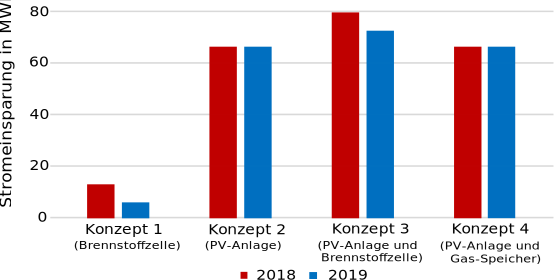
\includegraphics[scale=1]{Figures/Stromverbrauch_Sim_2}
		\caption{Vergleich der Simulationsergebnisse für den Jahresstromverbrauch des aktuellen Systems und der Konzepte samt Angabe der Stromeinsparungen im Vergleich zum aktuellen System.}
\label{fig:Strom}	
\end{figure}

\begin{table}[htb]
		\centering
		\caption{Vergleich der Stromeinsparungen, Einspeisung und Gaseinsparung der Systemkonzepte (Im erste Block sind die Daten für die Bedarfsverläufe aus 2018 und im zweite die Daten für die Bedarfsverläufe aus 2019 angegeben).}
		\begin{tabular}{l c c c}
		\toprule 
		& Stromeinsparungen & Einspeisung & Gaseinsparung
		\\
	    & in MWh & in MWh & in MWh\\
		\midrule
		Konzept 1 & $12,857$ &    -    & $14,083$\\
		Konzept 2 & $66,296$ & $4,313$ &    -    \\
		Konzept 3 & $79,637$ & $4,313$ & $14,032$\\
		Konzept 4 & $66,296$ & $4,313$ &    -    \\
		\midrule
		Konzept 1 & $5,858$  &    -    & $6,620$\\
		Konzept 2 & $66,295$ & $4,313$ &    -   \\
		Konzept 3 & $72,489$ & $4,313$ & $6,526$\\
		Konzept 4 & $66,295$ & $4,313$ &    -   \\
		\bottomrule
		\end{tabular}
		\label{tb:ErgebnisseSim}
\end{table}	
\FloatBarrier

\paragraph{Kapitalwerte der Systemkonzepte}\ \\
Die Kapitalwerte werden mithilfe der in \ref{Apx:Kapitalwert} angegebenen Parameter berechnet. In Abbildung \ref{fig:Kapitalwerte} werden die Kapitalwerte der Systemkonzepte graphisch gegenübergestellt, in Tabelle \ref{tb:Kapitalwerte} sind die Investitionen sowie jährliche Einnahmen und Ausgaben angegeben.\\

Für die Investition in eine Brennstoffzelle ergibt sich ein Kapitalwert von $5.\SI{847}{\sieuro}$ für den an 2018 angelehnten Prozessgasbedarf, mit den Daten für 2019 ergibt sich ein Kapitalwert von $-15.\SI{338}{\sieuro}$. Die Investition ist somit anhand des Kapitalwerts als tendenziell negativ zu bewerten. Um die Aussagekraft der Bewertung zu erhöhen, ist es sinnvoll, die Wahrscheinlichkeiten der beiden simulierten Szenarien abzuschätzen und dies in die Bewertung mit einfließen zu lassen. Für den Fall, dass in Zukunft mit steigendem Wasserstoffüberschuss zu rechnen ist, könnte sich die Investition in eine Brennstoffzelle als wirtschaftlich sinnvoll herausstellen.\\

Einen verbesserten Ansatz könnte die Installation einer Brennstoffzelle mit einer kleineren Zellfläche in Kombination mit einem Wasserstoffspeicher darstellen. Dadurch kann bei einer nahezu gleichbleibenden Stromeinsparung eine deutliche Verminderung der Investitionen erreicht werden, was durch eine überschlägige Berechnung verdeutlicht werden soll:\\
Bei den betrachteten Verläufen des Prozessgasbedarfs beträgt der maximal denkbare Überschuss an Wasserstoff ungefähr $\SI{5,3}{\kg}$ (In maximal $\SI{2}{\hour},\SI{45}{\minute}$ pro Tag wird überschüssiger Wasserstoff produziert und der maximale Stoffmengenstrom beträgt $\SI{0,2643}{\mol\per\s}$). Wird die Umwandlung des Wasserstoffs  nicht zeitgleich, sondern über den Tag verteilt vollzogen, reichen  $\frac{\SI{2}{\hour},\SI{45}{\minute}}{\SI{24}{\hour}} =  \SI{11,5}{\%}$ der im aktuellen Konzept veranschlagten Maximalleistung aus, um den Wasserstoffüberschuss vollständig zu nutzen. Dadurch sinkt die Investition der Brennstoffzelle auf $5.\SI{250}{\sieuro}$ (siehe \ref{Apx:Kapitalwert}). Investitonen in einen Wasserstoffspeicher können, wie in \ref{Apx:Kapitalwert} angegeben, mit $\SI{594}{\sieuro\per\kg_{H2}}$ abgeschätzt werden. Somit ergeben sich Gesamt-Investitionen von $\SI{8.400}{\sieuro}$, was einem Viertel der Investitionen des simulierten 
Brennstoffzellen-Konzepts entspricht. Da durch den zusätzlichen Betrieb des Speichers mit steigenden Betriebskosten und zusätzlichem Stromverbrauch zu rechnen ist, soll an dieser Stelle auf eine Berechnung des Kapitalwerts verzichtet werden. Allerdings zeigt die Abschätzung, dass durch die Kombination mit einem Gasspeicher mit einer deutliche Verbesserung hinsichtlich des Kapitalwerts zu rechnen ist.\\

Die Investition in eine PV-Anlage ergibt unabhängig vom verwendeten Bedarfsverlauf einen Kapitalwert von $84.\SI{726}{\sieuro}$. Die Bewertung der Wirtschaftlichkeit der Investition anhand des Kapitalwerts fällt also positiv aus.\\ 

Dies trifft auch auf die Kombination aus PV-Anlage und Brennstoffzelle zu, für die sich Kapitalwerte von $91.\SI{824}{\sieuro}$ und $70.\SI{220}{\sieuro}$ ergeben.
Es ist aber zu beachten, dass verglichen mit Konzept 2 die Mehrinvestition in eine Brennstoffzelle gemessen am Kapitalwert keinen deutlichen Mehrwert mit sich bringt. So erhöht sich der Kapitalwert für das Szenario 2018 bezogen auf die gesteigerten Investitionen nur unwesentlich und im Szenario 2019 sinkt der Kapitalwert durch die Mehrinvestition in eine Brennstoffzelle.\\

Zusammenfassend lässt sich daher sagen, dass nach Aussage des Kapitalwerts die Investition in eine PV-Anlage lohnenswert ist. Die ökonomische Bewertung der Brennstoffzelle hängt von dem prognostizierten Prozessgasverbrauch ab, fällt aber tendenziell negativ aus. Optimierungen des Brennstoffzellen-Konzepts versprechen aber deutliche Verbesserungen im Hinblick auf die ökonomische Bewertung.

\begin{figure}[h]
	\centering
		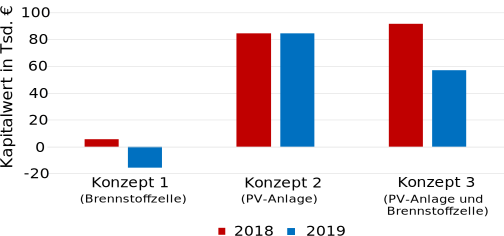
\includegraphics[scale=1]{Figures/Kapitalwerte}
		\caption{Kapitalwerte der Systemkonzepte.}
\label{fig:Kapitalwerte}	
\end{figure}

\begin{table}[htb]
		\centering
		\caption{Kapitalwerte der Konzepte sowie Kosten, die in die Berechnung einfließen (Im erste Block sind die Daten für die Bedarfsverläufe aus 2018 und im zweite die Daten für die Bedarfsverläufe aus 2019 angegeben).}
		\begin{tabular}{l c c c c}
		\toprule
		 & Investitionen & Einnahmen & Ausgaben & Kapitalwert\\
		& in € & in € & in € & in €\\
		Formelzeichen & $I_0$ & $Z_{ein}$ & $Z_{aus}$ & C\\
		\midrule
		Konzept 1 & $ 33.286$ & $ 3.550,63$ & $  259,71$ & $ 5.846,72$\\
		Konzept 2 & $ 80.352$ & $15.087,43$ & $1.205,00$ & $84.725,62$\\
		Konzept 3 & $113.638$ & $18.743,31$ & $1.464,71$ & $91.823,88$\\
		\midrule
		Konzept 1 & $ 33.286$ & $ 1.627,71$ & $  118,33$ & $-15.337,78$\\
		Konzept 2 & $ 80.352$ & $15.087,43$ & $1.205,00$ & $ 84.725,62$\\
		Konzept 3 & $113.638$ & $16.785,12$ & $1.323,33$ & $ 70.219,98$\\
		\bottomrule
		\end{tabular}
		\label{tb:Kapitalwerte}
\end{table}	

\FloatBarrier

\paragraph{CO2-Einsparungen der Systemkonzepte}\ \\
Die benötigten Parameter zur Berechnung der \ce{CO2}-Einsparungen sowie ihre Herleitung sind in \ref{Apx:CO2} aufgelistet. In Abbildung \ref{fig:CO2Einsparungen} werden die Einsparungen graphisch gegenübergestellt, die Bestandteile der Berechnung sind in Tabelle \ref{tb:CO2Einsparungen} aufgelistet.\\

Für die Verwendung einer Brennstoffzelle ergeben sich \ce{CO2}-Einsparungen von $\SI{8,0}{\tonne}$ für den an 2018 angelehnten Prozessgasbedarf, mit den Daten von 2019 werden $\SI{3,6}{\tonne}$ \ce{CO2} eingespart. Die Verwendung einer PV-Anlage im Energiesystem führt zu \ce{CO2}-Einsparungen von $\SI{24,8}{\tonne}$, bei einer Kombination von PV-Anlage und Brennstoffzelle liegen die \ce{CO2}-Einsparungen bei $\SI{32,9}{\tonne}$ beziehungsweise bei $\SI{28,5}{\tonne}$.\\

Alle drei Systemkonzepte versprechen somit eine Senkung der jährlichen \ce{CO2}-Emissionen. Die Einsparungen bei Verwendung der PV-Anlage sind dabei je nach Szenario $\SI{310}{\%}$ beziehungsweise $\SI{680}{\%}$ höher als die Einsparungen bei Verwendung einer Brennstoffzelle. 


\begin{figure}[h]
	\centering
		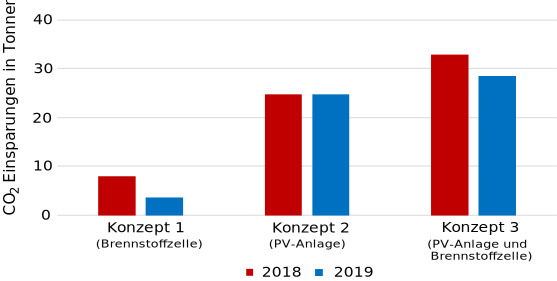
\includegraphics[scale=1]{Figures/CO2Einsparungen}
		\caption{ \ce{CO2}-Einsparungen der Systemkonzepte.}
\label{fig:CO2Einsparungen}	
\end{figure}

\begin{table}[htb]
		\centering
		\caption{\ce{CO2}-Einsparungen der Systemkonzepte sowie Einsparungen elektrischer Energie, Gaseinsparungen und bei der Produktion der Komponenten entstehende \ce{CO2}-Emissionen (Im erste Block sind die Daten für die Bedarfsverläufe aus 2018 und im zweite die Daten für die Bedarfsverläufe aus 2019 angegeben).}
		\begin{tabular}{l c c c c}
		\toprule
		 & Eisp. el. Energie & Gaseinsp. & \ce{CO2}-Em. der Prod. & \ce{CO2}-Einsp. \\
		& in MWh & in MWh & in Tonnen & in Tonnen\\
		Formelzeichen & $\Delta P_{el}$ & $\Delta Q$ & $\Delta m_{Prod.}$ & $\Delta m_{\ce{CO2}}$\\
		\midrule
		Konzept 1 & $12,957$ & $14,083$ & $0,038$ & $ 7,992$\\
		Konzept 2 & $70,609$ &    -     & $3,530$ & $24,784$\\
		Konzept 3 & $83,950$ & $14,032$ & $3,568$ & $32,919$\\
		\midrule
		Konzept 1 & $ 5,858$ & $6,620$ & $0,756$ & $ 3,643$\\
		Konzept 2 & $70,609$ &    -    & $3,530$ & $24,784$\\
		Konzept 3 & $76,802$ & $6,526$ & $3,568$ & $28,542$\\
		\bottomrule
		\end{tabular}
		\label{tb:CO2Einsparungen}
\end{table}

 
\chapter{Fazit und Ausblick}
\label{cha:Fazit}
In der vorliegenden Arbeit wird untersucht, ob das Wasserstoff-Energiesystem eines Quarzglasherstellers  


 ein Modell für Elektrolyseure und Brennstoffzellen in Modelica entwickelt. Das Modell wird anhand von Kennwerten aus Datenblättern parametriert und ist darüber hinaus in der Lage, Zellen verschiedener Technologien zu modellieren.\\

Aus der Validierung der Modelle geht hervor, dass sie für die im Rahmen dieser Arbeit angestrebte Untersuchungen ausreichend genaue Ergebnisse liefern: Bei der für die Simulation gewählten Betriebstemperatur liegen die Abweichungen der Polarisationskurve des alkalischen Elektrolyseurs bei unter $\SI{3,5}{\%}$, für die PEM-Brennstoffzelle ergeben sich Abweichungen von durchschnittlich $\SI{5,3}{\%}$.\\
Für einen PEM-Elektrolyseur werden Abweichungen von unter  $\SI{0,5}{\%}$ zu Messwerten aus der Literatur verzeichnet.\\
Bei den beiden PEM-Zellen nimmt die Genauigkeit des Modells außerhalb des gewählten Temperaturbereichs stark ab. 
---------- folgenden Absatz hier oder später? ------------
Daher wird empfohlen wie von \citet{falcao_review_2020} oder \citet{milewski_modeling_2014} präsentiert, eine Approximation des Temperatureinflusses auf die Fitting-Parameter in das Modell aufzunehmen. Zudem verspricht die getrennte Parametrierung von Elektrolyseur und Brennstoffzelle eine weitere Verbesserung der Ergebnisse.\\

Als Erweiterungen des Wasserstoff-Energiesystems des Quarzglasherstellers werden folgende Komponenten betrachtet: Eine Brennstoffzelle zur Nutzung des Wasserstoffüberschusses durch Kraft-Wärme-Kopplung, eine PV-Anlage und ein Gasspeichers zum Einspeichern von Solarstrom-Überschuss. Zur Bewertung der Systemkonzepte werden der Kapitalwert und die $\ce{CO2}$-Einsparungen berechnet.\\
Die ökonomische Bewertung der Brennstoffzelle fällt tendenziell negativ aus: Abhängig vom prognostizierten Prozessgasbedarf liegt der Kapitalwert zwischen $-15.388$ und $5.\SI{847}{\sieuro}$. Aus ökologischer Sicht stellt die Installation der Brennstoffzelle eine Verbesserung dar - es ergeben sich $\ce{CO2}$-Einsparungen von $3,6$ bis $\SI{8}{\tonne}$.\\ 
Die PV-Anlage wird als sinnvoll Investition gewertet, da der Kapitalwert mit $84.\SI{726}{\sieuro}$ klar positiv ausfällt (Der Kapitalwert übersteigt dabei die Anfangsinvestitionen). Auch aus ökologischer Sicht wird die PV-Anlage verglichen mit der Brennstoffzelle positiver eingestuft: Die simulierten $\ce{CO2}$-Einsparungen sind mit $\SI{24,8}{\tonne}$ um den Faktor 3 bis 6 höher.\\

Für folgende Arbeiten wird eine Validierung des Modells bei verschiedenen Druckniveaus empfohlen.\\

Um die Rechenzeit der Simulation gering zu halten wird in dieser Arbeit auf eine Simulation des thermischen Verhaltens der Elektrolysezelle verzichtet, allerdings kann diese bei Bedarf aus dem Brennstoffzellenmodell übernommen werden. Daraus könnte bewertet werden, ob eine Nutzung der Abwärme der Elektrolysezelle sinnvoll ist.
Eine weitere Möglichkeit zur Ausweitung des Modells sind dynamische Vorgänge, die in dieser Arbeit aufgrund der großen Zeitschritte der Simulation nicht beachtet wurden (Ausführlichere Begründung in \ref{subsec:Modellierung der Zelle}). Um diese zu berücksichtigen, kann die Instaionarität der Zelltemperatur in der Energiebilanz (Gleichung \ref{gl:Energiebilanz}) beibehalten werden.\\

Einige Autoren nutzten daher Approximationen, um den Verlauf der Parameter $\alpha$ und $i_0$ über der Temperatur im Modell zu berücksichtigen . Für die Modellierung von PEM-Zellen verspricht dies eine 
Steigerung der Genauigkeit bei niedrigen Temperaturen. Ob diese Maßnahme die Genauigkeit der Modellierung von alkalischen Zellen erhöht ist unklar, da die Validierungsergebnisse des alkalischen Elektrolyseurs keine signifikante Steigerung der Abweichungen bei zu- oder abnehmenden Temperaturen dokumentieren.\\

In folgenden Arbeiten sollte daher untersucht werden, ob weitere Messreihen den unterschiedlichen Temperatureinfluss auf die Polarisationskurven bestätigen. Dies würde im Modell gegebenenfalls eine Unterscheidung bei der Berechnung der Verluste von Brennstoffzellen und Elektrolyseuren erfordern.\\


%-----------------------------------------------------------------------------
% Bibliography
%-----------------------------------------------------------------------------
\clearpage
\refstepcounter{Hilfszaehler}
\addcontentsline{toc}{chapter}{\bibname}
\protect\bibliographystyle{plainnat} % This style is not mandatory. Another would be e.g. natdin.
\bibliography{Literature}


%-----------------------------------------------------------------------------
% Appendix		 	     
%-----------------------------------------------------------------------------
\cleardoublepage
\FloatBarrier	% Prevents figures/tables to move to appendix
\addtocontents{toc}{\protect\setcounter{tocdepth}{2}}
%Prevents Appendix sections to show in the TOC if you set the number to 0

\captionsetup{list=no}	
% Prevents captions of figures/tables in appendix t appear in the list of figures and tables

\begin{appendix}
\newpage\thispagestyle{empty}~
\vfill{}\vspace{-1\parskip}
\begin{center}\textsf{\textbf{\huge \appendixName}}\end{center}{\huge \par}
\vfill{}
~
%TODO	%%% ADD YOUR APPENDIX CHAPTERS HERE %%%
\newpage
\chapter{Parametrierung der Modelle}
\label{Apx:Modelle}
\paragraph{Alkalischer Elektrolyseur}\ \\
Vom Hersteller ist die maximale Wasserstoffproduktion mit $\SI{21,33}{\Nmc\per\hour}$ angegeben \citep[S. 50]{noauthor_bedienungs-_nodate}, dies entspricht $\SI{0,2643}{\mol\per\s}$. Über den Zusammenhang der von $i$ und $\dot{n}_{H_2O}$ (Gleichung \ref{gl:n_i}) und der maximalen Stromdichte von $\SI{0,5}{\A\per\cm\squared}$ wird daher eine Zellfläche von $\SI{10,2}{\m\squared}$ angenommen.\\
Die Elektrolyt-Konzentration ist mit $\SI{20}{\%}$ angegeben \citep[S. 36]{noauthor_bedienungs-_nodate}, was bei Natronlauge $\SI{6,095}{\mol\per\l}$ entspricht \citep{periodensystem-online_dichtewerttabelle_nodate-1}\\
Für den Parameter $\alpha$ wurde der von \citet{milewski_modeling_2014} für die Kathode angegebene Wert verwendet. Weil \citet{milewski_modeling_2014} die Aktivierungsverluste mit dem Faktor $2,3026$ multipliziert, ist der verwendete Wert für $\alpha$ wie folgt bereinigt:
\begin{align*}
\frac{1}{\alpha} = &\frac{2.3026}{\alpha _{milewski}}\\
\alpha = &\frac{\alpha _{milewski}}{2,3026}\\
	   = &\frac{0,39}{2,3026} = 0,17
\end{align*}

\paragraph{PEM-Brennstoffzelle}\ \\
Die Zellfläche der Brennstoffzelle wurde aus der Zellfläche des Elektrolyseurs und dem Verhältnis der maximalen Stromdichte abgeleitet: 
\begin{align*}
A_{Brennstoffzelle} = &A_{Elektrolyseur} \cdot \frac{i_{max, pem}}{i_{max, alk}}\\
                    = &\SI{10,2}{\m\squared} \cdot \frac{\SI{2}{\A\per\cm\squared}}{\SI{0,5}{\A\per\cm\squared}}\\
	   				= &\SI{2,55}{\m\squared}
\end{align*}
Nach den Simulationsergebnisse liegt die maximale elektrische Leistung der Brennstoffzelle bei $\SI{24,475}{\kilo\W}$.\\
Der Parameter $C_{th}$ ist \citet{webster_implementation_2019} entnommen und wurde über die Zellfläche skaliert:
\begin{align*}
C_{th} = &C_{th,webster} \cdot \frac{A}{A_{webster}}\\
       = &\SI{14,97}{\W\per\K} \cdot \frac{\SI{2,55}{\m\squared}}{\SI{1,74}{\m\squared}}\\
	  = &\SI{21,94}{\W\per\K}
\end{align*}

\chapter{Systemkonzepte}
\label{Apx:Systemkonzepte} 
\paragraph{Gasbedarf}\ \\
Für die Monate Juni bis August wird angenommen, dass keine Heizwärme benötigt wird. Der maximale Gasverbrauch eines Tages in diesem Zeitraum  liegt bei $\SI{18,8}{\m\cubic} \cdot \SI{11,4}{\kiloWh\per\cubic\m} = \SI{214,32}{\kiloWh\per\cubic\m}$ (Brennwert 2020 nach Gasabrechnung G 685 - Regionetz \citep{regionetz_gasabrechnung_nodate}).\\
Von dem Tagesgasverbrauch wird dieser Wert abgezogen und das Ergebnis als zum Heizen benötigte Gasmenge pro Tag angenommen (Weil Elektrolyseur und Brennstoffzelle ausschließlich während der Arbeitszeit (ca. 6.30-16.30) betrieben wird ausschließlich die Gasmenge während der Arbeitszeit in Betracht gezogen).\\

\paragraph{Prozessgasverbrauchswerte}\ \\
Wasserstoff und Sauerstoff wurden vom Kunden in Bündeln je 12 Flaschen mit einem Volumen von $\SI{50}{\l}$ und einem Druck von $\SI{300}{\bar}$ gekauft (In Tabelle \ref{tb:Einkauf} sind die Einkaufsmengen für die Jahre 2018 und 2019 angegeben). Nach dem idealen Gas Gesetz ergeben sich daraus die angegebenen Stoffmengen bei der Standardtemperatur von $\SI{298,15}{\K}$.

\begin{table}[ht]
		\centering
		\caption{Gekaufte Menge an Wasserstoff und Sauerstoff für die Jahre 2018 und 2019.}
		\begin{tabular}{l c c}
		\toprule
		 & Anzahl an Bündeln & Stoffmenge\\
		\midrule
		Wasserstoff 2018 & 105 & $\SI{775420}{\mol}$\\
		Sauerstoff 2018 & 86 & $\SI{635106}{\mol}$\\
		Wasserstoff 2019 & 66 & $ \SI{487407}{\mol}$\\
		Sauerstoff 2019 & 47 & $\SI{347093}{\mol}$\\
		\bottomrule
		\end{tabular}
		\label{tb:Einkauf}
\end{table}	

Zur Berechnung des Jahressauerstoffbedarfs der Datensätze wird die tägliche Bedarfszeit mit der Anzahl der Arbeitstage im Jahr (mit 245 angenommen) und der durchschnittlichen Stoffmengenproduktion ($\SI{0,2643}{\mol\per\s} \cdot \SI{75}{\%} / 2 = \SI{0,0991}{\mol\per\s}$ für Sauerstoff und $\SI{0,2643}{\mol\per\s} \cdot \SI{75}{\%} = \SI{0,1982}{\mol\per\s}$ für Wasserstoff) multipliziert. 

\begin{table}[ht]
		\centering
		\caption{Berechnung des Jahressauerstoff- und wasserstoffverbrauchs für Datensätze 1 und 2.}
		\begin{tabular}{l c c c}
		\toprule
		 & Bedarfszeit & Jahresverbrauch & Abweichung zum Realwert\\
		\midrule
		Datensatz 1 $H_2$ & $\SI{4}{\hour},\SI{30}{\minute}$ & $\SI{786775}{\mol}$ & $\SI{1,5}{\%}$\\
		Datensatz 1 $O_2$ & $\SI{7}{\hour},\SI{15}{\minute}$ & $\SI{633775}{\mol}$ & $\SI{0,2}{\%}$\\
		Datensatz 2 $H_2$ & $\SI{2}{\hour},\SI{45}{\minute}$ & $\SI{480795}{\mol}$ & $\SI{0,5}{\%}$\\
		Datensatz 2 $O_2$ & $\SI{4}{\hour}$ & $ \SI{349669}{\mol}$ & $\SI{0,7}{\%}$\\
		\bottomrule
		\end{tabular}
		\label{tb:VerbrauchSimulation}
\end{table}	

\chapter{Parameter zur Berechnung des Kapitalwerts}
\label{Apx:Kapitalwert}

\begin{table}[ht]
		\centering
		\caption{Parameter der Kapitalwertberechnung.}
		\begin{tabular}{l c c}
		\toprule
		Kalkulationszeitraum & $n$ & $\SI{20}{\a}$ \citep{von_appen_optimale_2015}\\ 
		Kalkulatorischer Zinssatz & $r$ & $\SI{5,56}{\percent}$ \cite{gpanrw_kalkulatorischer_2021}\\
		Strompreis & $z_{netzbezug}$ & $\SI{22,26}{\cent\per\kiloWh}$ \citep{eon_energie_ihr_2021}\\
		Einspeisevergütung & $z_{eispeisung}$ & $\SI{7,65}{\cent\per\kiloWh}$ \citep{bna_bundesnetzagentur_2021}\\
		Gaspreis & $z_{gas}$ & $\SI{4,89}{\cent\per\kiloWh}$ \citep{eon_energie_gewerbegas_2021}\\
		Investitionskosten der PV-Anlage & $I_{PV}$ & $80.\SI{352}{\sieuro}$ \citet{von_appen_optimale_2015}\\
		Jährliche Wartungskosten der PV-Anlage & $Z_{PV}$ & $1.\SI{205}{\sieuro}$ \citet{von_appen_optimale_2015}\\
		Investitionskosten der Brennstoffzelle & $I_{BZ}$ & $ 33.\SI{286}{\sieuro}$ \citep{jungbluth_kraft-warme-kopplung_2012}\\
		Jährliche Betriebskosten der Brennstoffzelle & $z_{BZ}$ & $\SI{2,02}{\cent\per\kiloWh}$ \citep{jungbluth_kraft-warme-kopplung_2012}\\
		Speicherkosten pro Kilogramm Wasserstoff & $z_{Speicher}$ & $\SI{891}{\sieuro\per\kg}$ \citep{schill_vergleich_2018}\\
		\bottomrule
		\end{tabular}
		\label{tb:ParameterKapitalwert}
\end{table}
	
Der Betrachtungszeitraum wird, wie auch bei \citet{von_appen_optimale_2015} auf $20$ Jahren angesetzt. Als kalkulatorische Zinssatz wird der in \cite{gpanrw_kalkulatorischer_2021} für das Jahr 2020 als Obergrenze angegebene Wert übernommen. Der Strom- und Gaspreis sind \citet{eon_energie_ihr_2021} (für einen Jahresbedarf von $\SI{866.860}{\kiloWh}$) und \citet{eon_energie_gewerbegas_2021} (für einen Jahresbedarf von $\SI{27.224}{\kiloWh}$) entnommen. Die Einspeisevergütung ergibt sich aus den Angaben der Bundesnetzagentur \citep{bna_bundesnetzagentur_2021} für Solarstromanlagen mit einer Peakleistung bis zu $\SI{40}{\kiloWh}$ (Installation ab dem 01.07.2021). \\ 
\citet[S.3]{von_appen_optimale_2015} geben als Investitionskosten für PV-Anlagen bezogen auf die installierte Fläche: $\SI{150}{\sieuro\per\m\squared}$ an. Mit 372 Module a $\SI{1,44}{\m\squared}$ ergeben sich Investitionskosten von $SI{150}{\sieuro\per\m\squared} \cdot\SI{1,44}{\m\squared} \cdot 372 = \SI{80.352}{\sieuro}$. Die jährliche Wartungskosten liegen nach \citet{von_appen_optimale_2015} bei $\SI{1,5}{\%}$ der Investitionskosten.\\
Die Investitionskosten der Brennstoffzelle betragen nach \citet[S. 74]{jungbluth_kraft-warme-kopplung_2012}  $\SI{1360}{\sieuro\per\kilo\W}$ bei einer elektrischen Peakleistung von $\SI{24,475}{\kiloW}$ (Maximalwert der Brennstoffzellen-Ausgangsleistung der Simulation). Die Betriebskosten gibt er mit $z_{BZ} = \SI{2,02}{\cent\per\kiloWh}$ an (Nach den Simulationsergebnissen beträgt die Jahresleistung der Brennstoffzelle $12.\SI{857}{\kiloWh}$ für 2018 beziehungsweise $5.\SI{858}{\kiloWh}$ für 2019.\\		 
Speicherkosten für Wasserstoff liegen nach \citet{schill_vergleich_2018} zwischen $10$ bis $\SI{30}{\sieuro\per\kiloWh}$ bezogen auf den Brennwert. Daraus ergeben sich Speicherkosten von $\frac{\SI{15}{\sieuro\per\kiloWh} \cdot \Delta H^0_R}{M_{H_2}} = \SI{594}{\sieuro\per\kg_{H2}}$.\\
Da ein Speicher für $\ce{H2}$ und $\ce{O2}$ im Stoffmengenverhältnis $2:1$ benötigt wird, werden spezifische Speicherkosten von $z_{Speicher} = 1,5 \cdot \frac{\SI{15}{\sieuro\per\kiloWh} \cdot \Delta H^0_R}{M_{H_2}} = \SI{891}{\sieuro\per\kg_{H2}}$ angenommen.\\	

Für die Überschlagsrechnung des optimierten Brennstoffzellen-Konzepts wird von einer Maximalleistung von $\SI{24,475}{\kiloW} \cdot \SI{11,5}{\%} = \SI{2,8}{\kiloW}$ gerechnet. Nach \citet[S. 74]{jungbluth_kraft-warme-kopplung_2012} ergeben sich dafür spezifischen Investitionskosten von $1.\SI{875}{\sieuro}$.

\chapter{Parameter zur Berechnung der CO2-Einsparungen}
\label{Apx:CO2}
\begin{table}[ht]
		\centering
		\caption{Parameter der $\ce{CO2}$-Einsparungen.}
		\begin{tabular}{l c c}
		\toprule
		 $\ce{CO2}$ Faktor Strommix & $m_{Strom}$ & $\SI{401}{\g\per\kiloWh}$ \citep{ortl_entwicklung_2020} \\
		 $\ce{CO2}$ Faktor Erdgas & $m_{Gas}$ & $\SI{201,24}{\g\per\kiloWh}$ \citep{redaktionsassistenz_2_co2-emissionsfaktoren_2016}\\
		 $\ce{CO2}$ PV-Strom & $m_{PV}$ &$\SI{50}{\g\per\kiloWh}$ \citep[S. 48]{wirth_aktuelle_nodate}\\
		 $\ce{CO2}$ Brennstoffzelle & $m_{BZ}$ &$\SI{38,8}{\kg\per\a}$ \citep{miotti_integrated_2017}\\
		\bottomrule
		\end{tabular}
		\label{tb:ParameterCO2}
\end{table}

Für den $\ce{CO2}$ Faktor des Deutschen Strommix wurden Daten aus 2019 verwendet \citep{ortl_entwicklung_2020}. Die spezifischen $\ce{CO2}$-Emissionen von Erdgas lagen in Deutschland zwischen 2005-2014 bei konstant $\SI{55,9}{tonne}$-$\ce{CO2}$/TJ  \citep{redaktionsassistenz_2_co2-emissionsfaktoren_2016} was umgerechnet $\SI{201,24}{\g\per\kWh}$ ergibt.\\
Für die Herstellung der PV-Anlage und der Brennstoffzelle wurden Angaben für die Emissionen von $\ce{CO2}$-Äquivalent verwendet. Im Falle der PV-Anlage wurden die durchschnittlichen  Emissionen von Deutschem PV-Strom verwendet. 
Die Emissionen bei der Herstellung von Brennstoffzellen liegen nach \citet{miotti_integrated_2017} bei $\SI{2,47}{\tonne}$ bei einer Anlage mit einer elektrischen Leistung von $\SI{80}{\kiloW}$. Die spezifischen $\ce{CO2}$-Emissionen betragen demnach $\SI{30,9}{\kg\per\kiloW}$, wonach die in den Systemkonzepten eingesetzt Brennstoffzelle bei der Herstellung $\SI{756,3}{\kg}$-$\ce{CO2}$-Äquivalent verursacht. Für die Berechnung der $\ce{CO2}$-Einsparungen wird dieser Wert auf die angenommene Lebensdauer ($\SI{20}{\a}$) aufgeteilt.
\end{appendix}

\addtocontents{toc}{\protect\setcounter{tocdepth}{2}}
% Sets the TOC depth back to its original value



%-----------------------------------------------------------------------------
% Declaration of originality
%-----------------------------------------------------------------------------
\pagestyle{empty}
\clearpage
\iftoggle{thesis}{%
	\iftoggle{ingerman}{%
		\Large
\textbf{Eigenständigkeitserklärung}

\begin{normalsize}
Hiermit versichere ich, dass ich die vorliegende Arbeit selbstständig und ohne Benutzung anderer als der angegebenen Hilfsmittel angefertigt habe. Alle Stellen, die wörtlich oder sinngemäß übernommen sind, sind als solche kenntlich gemacht. Die Arbeit ist in gleicher oder ähnlicher Form noch nicht als Prüfungsarbeit eingereicht worden. Ich erkläre mich damit einverstanden, dass die vorliegende Arbeit in der Lehrstuhlbibliothek und Datenbank aufbewahrt und für den internen Gebrauch kopiert werden darf. \newline \newline


Aachen, \today \newline \newline

%TODO Name ergänzen
Tobias Jonathan Boschmann
\end{normalsize}
	}{%
		\Large
\textbf{Declaration of Originality}

\begin{normalsize}
I hereby declare that this thesis and the work reported herein was composed by and originated entirely from me. Information derived from the published and unpublished work of others has been acknowledged in the text and references are given in the list of sources. This thesis has not been submitted as exam work in neither the same nor a similar form. I agree that this thesis may be stored in the institutes library and database. This work may also be copied for internal use. \newline \newline


Aachen, \today \newline \newline

%TODO put your name here
YOUR NAME HERE
\end{normalsize}
	}
}{}



\end{document}